
\section{Pre-trained LLMs are Contextually Sparse} \label{sec:obs}
In this section, we present several key observations and theoretical understandings of sparsity in LLMs, upon which the \name{} design is based.
We first test the contextual sparsity hypothesis and verify that contextual sparsity exists in pre-trained LLMs in Section~\ref{sec:sparse_obs}. Then, we build an understanding of why contextual sparsity happens naturally even when LLMs are densely trained in Section~\ref{sec:obs_att_cluster}. Finally, we present an observation on residual connections and explain their relationship to contextual sparsity analytically in Section~\ref{sec:obs_slowly_changing}.

\begin{figure}[t]
  \centering
    \subfigure[Contextual sparsity in Attention Head]{
    \hspace{0mm}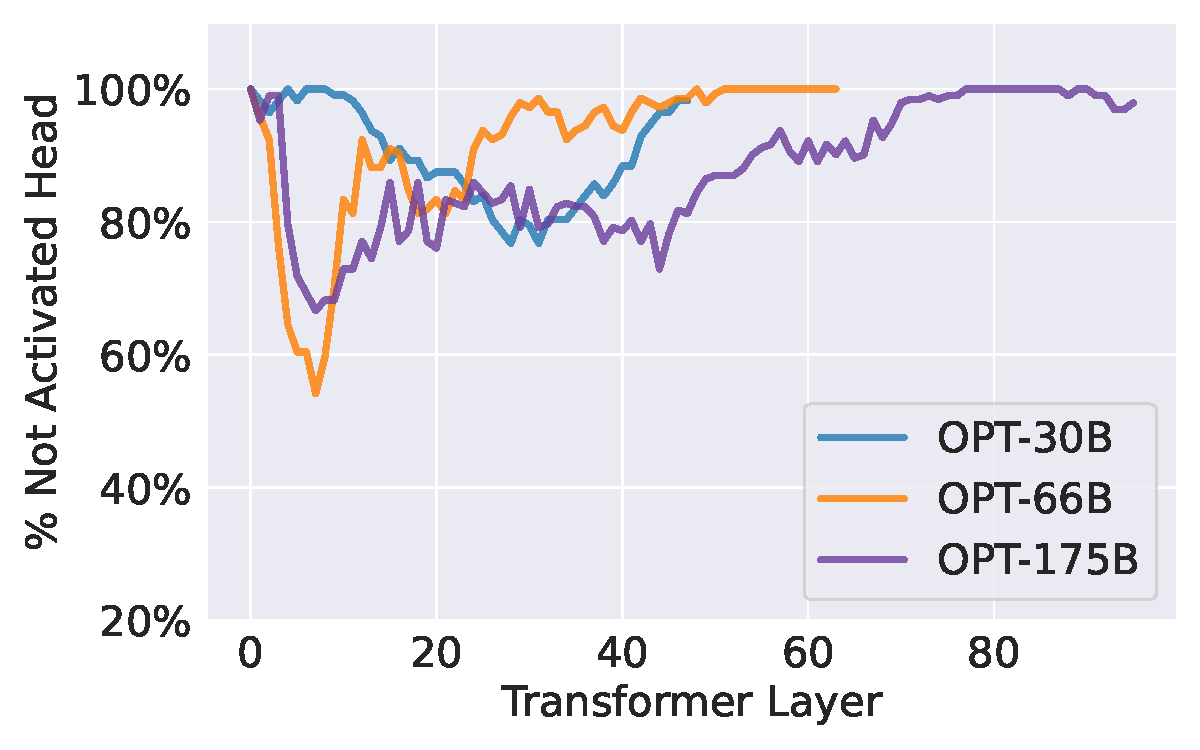
\includegraphics[width=0.36\textwidth]{figure/head_sparsity.pdf}
    \label{obs:175b-sparsity-att} 
  }\\
  \vspace{-2mm}
  \subfigure[Contextual sparsity in MLP Block]{
    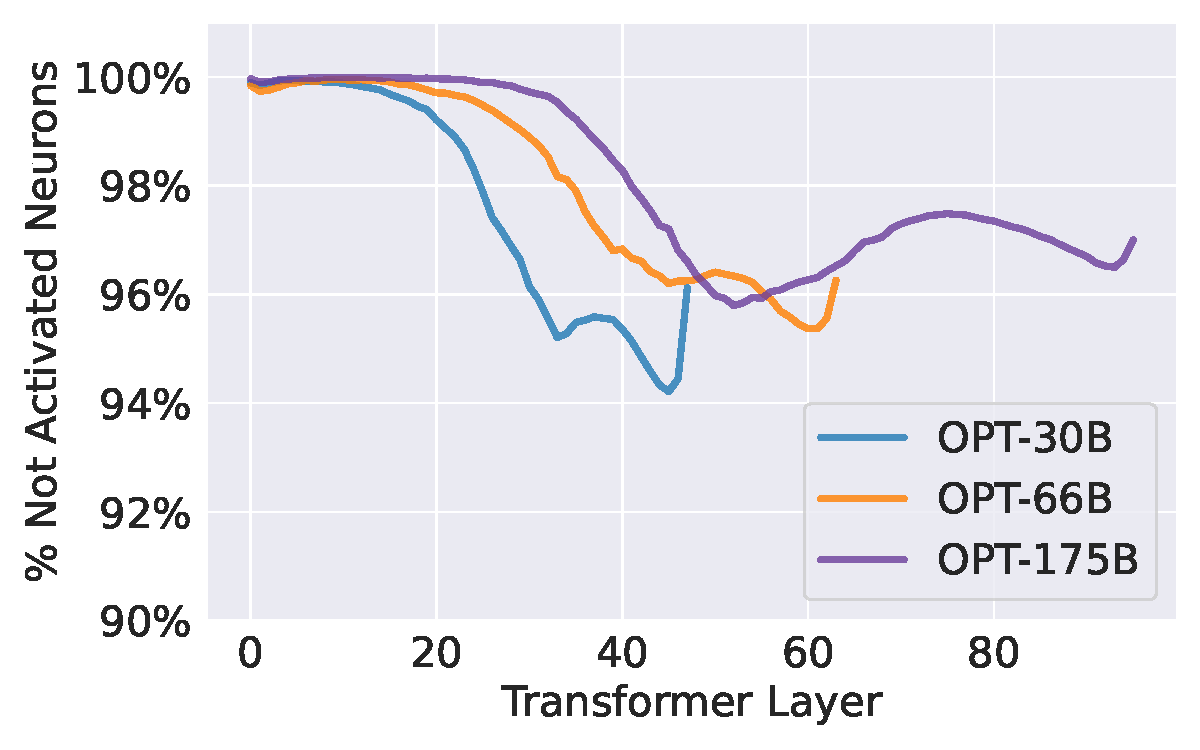
\includegraphics[width=0.36\textwidth]{figure/mlp_sparsity.pdf}
    \label{obs:175b-sparsity-mlp} 
  }
    \vspace{-2mm}
  \caption{ In Figure (a), we plot the percentage of not-activated attention heads. By only keeping heads that yield large output norms, we can silence over 80\% attention heads for a given token. In Figure (b), we plot the average sparsity we impose on MLP layers. We can zero out over 95\% of MLP parameters for a given token.}
    \vspace{-4mm}
  \label{observation:sparsity} 
\end{figure}

\subsection{Contextual Sparsity Hypothesis}
% \subsection{High Contextual Sparsity in MLP and Attention}
\label{sec:sparse_obs}
% Sparsity is a naturally occurring phenomenon in large language models. 
Inspired by prior pruning literature~\cite{molchanov2016pruning}, we find a surprisingly simple method is sufficient to study and verify our hypothesis. In this section, we describe the testing procedure, observation details, and insights of this study.   

\textbf{Verification:} Our test is performed on OPT-175B, 66B, and 30B models and various downstream datasets such as OpenBookQA~\cite{OpenBookQA2018} and Wiki-Text~\cite{merity2016pointer}. We find the contextual sparsity for every input example with two forward passes of the model. In the first pass, we record a subset of parameters, specifically which attention heads and MLP neurons yield large output norms for the input. In the second pass, each input example only uses the recorded subset of parameters for the computation. Surprisingly, these two forward passes lead to similar prediction or performance on all in-context learning and language modeling tasks.

\textbf{Observation:}  Figure~\ref{observation:sparsity} shows that on average, we can impose up to 80\% sparsity on attention heads and 95\% sparsity on MLP neurons. As mentioned in Section~\ref{sec:obs_computation}, OPT-175B model has $2\times$ MLP parameters than those of attention blocks. Therefore total sparsity here is around 85\%. Since these are all structured sparsity (heads and neurons), predicting them accurately could potentially lead to $7 \times$ speedup.   

\textbf{Insight:} It is intuitive that we can find contextual sparsity in MLP blocks at inference time because of their activation functions, e.g., ReLU or GeLU~\cite{pmlr-v119-kurtz20a}. Similar observations were made by~\cite{sanjiv}. However, it is surprising that we can find contextual sparsity in attention layers. Note that, finding contextual sparsity in attention is not the same as head pruning. We cross-check that different examples have different contextual sparsity. Although $80\%$ of the parameters are not included in the paths for a given example, they might be used by other examples. Next, we will try to understand why contextual sparsity exists in attention blocks.

% 

% Here, we summarize our findings on contextual sparsity~\ref{observation:sparsity}. 


% As shown in  over 95\% of parameters in the Expand MLP output zero values after the activation function, suggesting a high contextual sparsity ratio and a significant waste in compute.  In this Multi-Head-Attention Block, a given input is passed through multiple attention heads, and their outputs are concatenated together for output projection. At every head, a token will attend to every other token in the sequence, and the attention weight is decided based on the softmax probability. During training, each head is optimized for different sensitivities, like different convolution filters measure different characteristics~\cite {cordonnier2019relationship}. At each head, there may exist two outcomes depending on the head behavior: (1) the current token has high attention weights with a few tokens in the sequence, and (2) the current token has similar attention weights for the entire sequences. We consider the second situation as a sparsity head for this token because this token fails to find something it needs to pay attention to. In Figure~\ref{obs:sparsity-att}, we plot the percentage of the uniform head. Specifically, we calculate how many tokens are needed for the softmax score to accumulate to over 0.99. And we set 20\% as the threshold. We find that in the middle layers, over 80\% heads perform token mixing in a rather uniform manner, which suggests that all the sparse heads are performing rather similar computations.

% At the same time, a majority of neurons are activated, just by different input sequence. As for OPT-175b, we can barely find ``dead'' neurons can be pruned without any consequences after 40 layers.

% (3) \textit{Dead neurons at lower layers.} Some neurons in lower transformer layers never get activated for any input tokens, and thereby can be safely pruned without any consequences. It should be noted that the portion gets larger for larger models.

% Additionally, dynamic sparsity is prevalent across most layers.
% By dynamic sparsity, we mean that a majority of neurons are activated but by varying input tokens.

% shows that on average each token only activates 5\% rows (or columns) in FFN matrices and 10\% of attention heads. Furthermore, since token generation latency is one of the major challenges of LLM deployment for its token-by-token serial computation (details in Section~\ref{sec:related_work}), the above observation provides a huge opportunity to generate tokens $15\times$ faster.

\subsection{Token Clustering in Attention Layers}
\label{sec:obs_att_cluster}

In the previous section, we have verified that there exists contextual sparsity for a given input in LLMs. In this section, we try to understand the reason for such phenomena, especially in attention layers. We first show an in-depth observation of attention. Then we present a hypothesis that self-attentions are conceptually clustering algorithms. Last we show analytical evidence to support this hypothesis. 


\textbf{Observation:} Figure~\ref{fig:head_uniform} shows the attention map of three different heads from the same layer for an example input. The next token it should predict is ``Truck''. Darker color represents higher attention scores. We observe that the middle head is a relatively uniform token-mixing head while the top and bottom ones are ``heavy hitter'' attention heads (with high attention to ``like'' and ``shipping''). Unsurprisingly, only selecting heavy hitter heads but not uniform heads does not affect the prediction, since uniform heads do not model or encode important token interactions. In the next section, we will also explain in detail how the criteria for selecting uniform attention heads and heads with small output norms are highly correlated.    

\def\vone{\mathbf{1}}

\textbf{Hypothesis:} We hypothesize that the attention head is performing mean-shift clustering~\cite{derpanis2005mean}. 

Recall the notation defined in Section~\ref{sec:formulation}. For $i$-th head at current layer, $X = [x_1, \ldots, x_n]^{\top} \in \mathbb{R}^{n\times d}$ are the token embeddings in the previous time steps. $X W_i^K $ and $X W_i^V $ are the projection of embedding. For an input embedding $y$, the output $\tilde y_i = H_i(y)$, where $H_i(y)$ is defined in Eq.~\ref{eq:H_i_y}. 

\def\vm{\mathbf{m}}
For each $i \in [h]$, if we let $K_i(x_j,y) := \exp(y W_i^Q(W_i^K)^\top x_j)$ measure the similarity between $x_j$ and $y$, and define $m_i(y) := \frac{\sum_j K_i(x_j,y) x_j}{\sum_j K_i(x_j,y)}$, then we have $\tilde y_i =  m_i(y) W_i^V$. Further, if we set $W^V_i=I$ and consider the residue connection followed by layer norm, then in the next layer, the embedding $\hat y_i$ of the current token becomes $\hat y_i = \mathrm{Normalize}(y + \tilde y_i) = \mathrm{Normalize}(y + m_i(y))$, which has a fixed point $y = \gamma m_i(y)$ for any scalar $\gamma$. This iteration bears a resemblance to mean-shift clustering, which simply performs iteration $y \leftarrow m_i(y)$ until convergence. This has an obvious fixed point $y = m_i(y)$. 

Therefore, the self-attention head can be regarded as \emph{one mean-shift step} to push input embeddings of different tokens together, if they are already neighbors in a projection space specified by $W_i^Q (W_i^K)^\top $. Different heads learn different projection spaces to perform clustering. These dynamics explain the precise reason why token embeddings tend to cluster after going through more layers, resulting in high attention scores among cluster members, and low scores for non-members. Furthermore, the cluster patterns are different at different heads (More details in Appendix~\ref{sec:clustering understanding}).

The above analysis not only provides an understanding of why contextual sparsity exists naturally in pre-trained LLMs, but also inspires our design of ``similarity''-based sparsity prediction for \name{} in Section~\ref{sec:method}.  

%At head $i$, if the attention weights for a token $x$ are rather dense on a few tokens, it suggests that $x$ belongs to one cluster under head $i$'s clustering standard, and tokens in this cluster will have high attention weights on each other. 

\begin{figure}[]
 \vspace{-2mm}
  \centering
    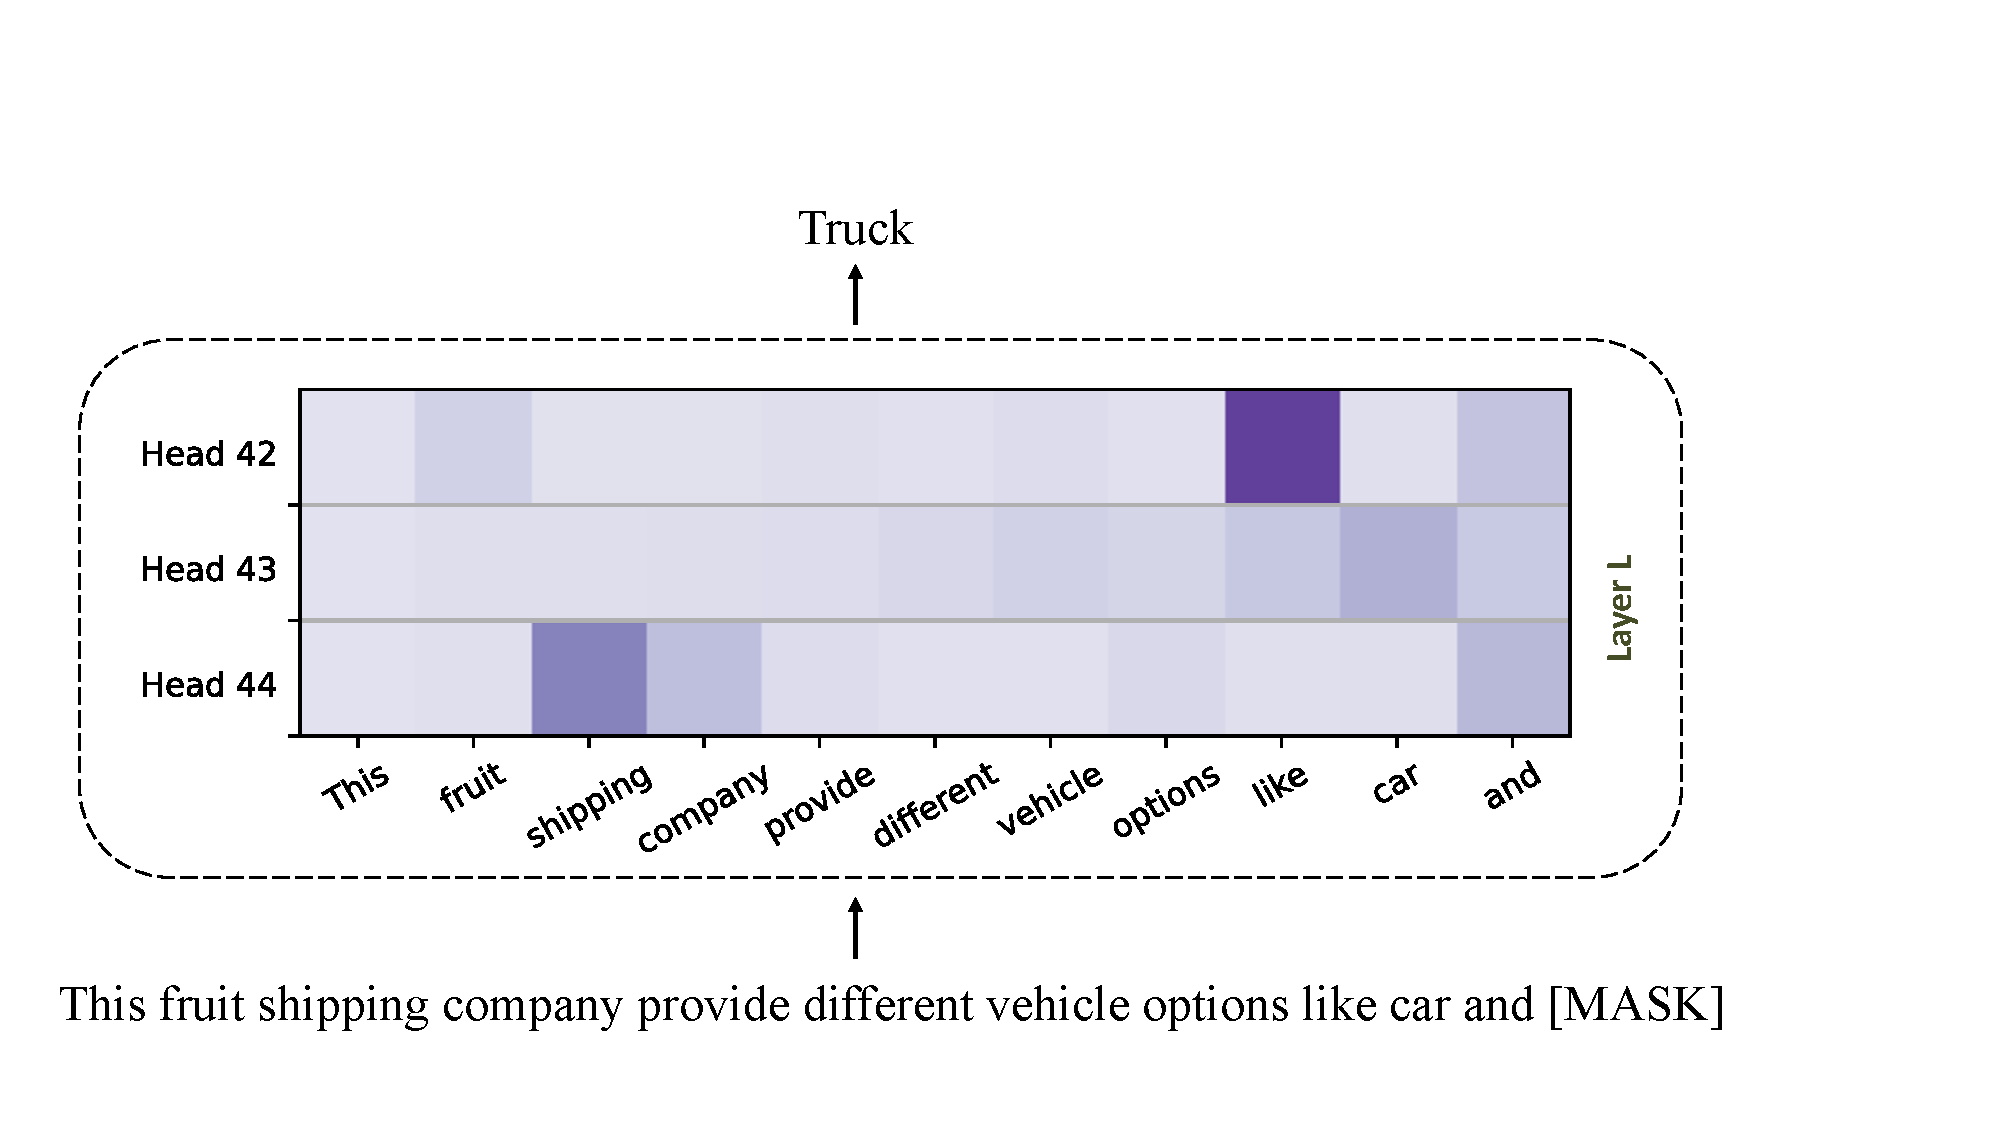
\includegraphics[width=0.47\textwidth]{figure/Attention_clustering.pdf}
    \vspace{-3mm}
  \caption{ We visualize the attention scores of three different heads for an exemplary sentence. Head 42 and Head 44 give heavy attention scores on particular tokens while Head 43 is more uniform.     }
  \label{fig:head_uniform} 
     \vspace{-4mm}
\end{figure}
% In the previous example that when generating the fifth token, it does not go through head 1 in layer 10: if when generating the sixth token, it is similar and highly correlated with the fifth one at layer 10, it will go through the same paths / heads and highly likely not going through head 1; if the sixth token is not similar or correlated with the fifth one, not attending with the fifth token does not lose too much information.

\subsection{Slowly Changing Embeddings across Layers}
\label{sec:obs_slowly_changing}

\begin{figure}[]
\vspace{-2mm}
  \centering
 \subfigure[Model Comparison]{
    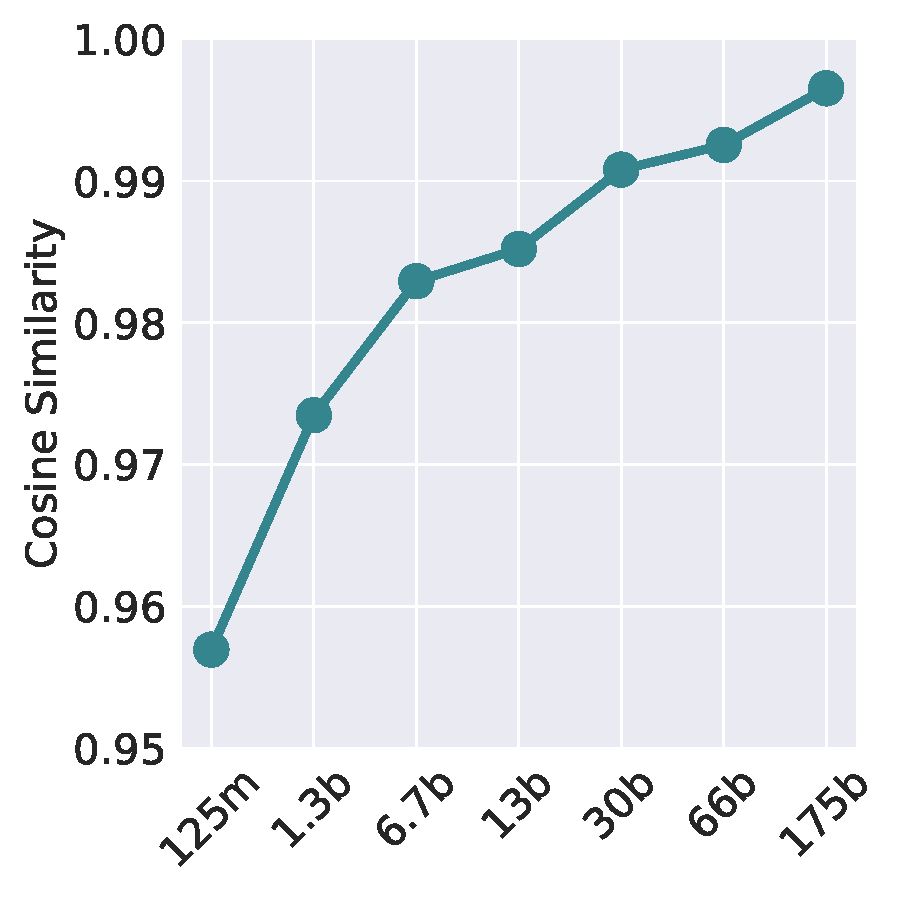
\includegraphics[width=0.22\textwidth]{figure/observation/cos_across_model.pdf}
    \label{obs:slowlyevoloving-all}
    }
  \subfigure[Across Layer]{
    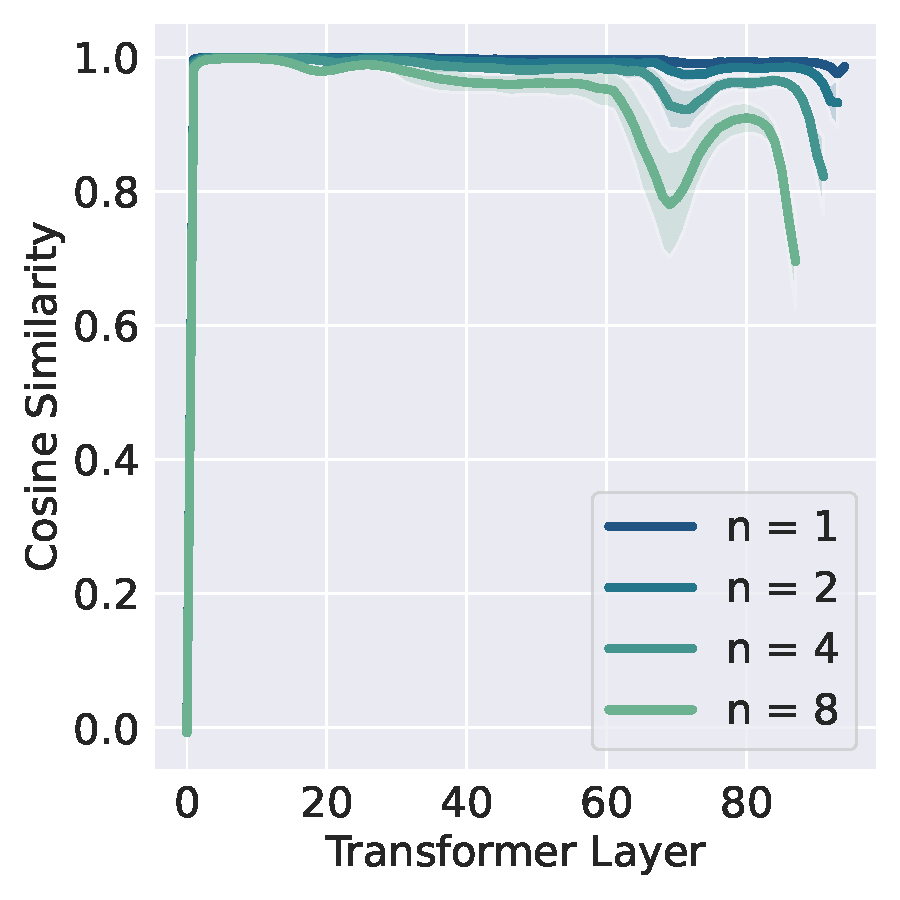
\includegraphics[width=0.22\textwidth]{figure/observation/175b_between_layer_cos.pdf}
    \label{obs:slowlyevoloving-175b}
  } \\
  \vspace{-4mm}
    \subfigure[Residual Around Attention]{
    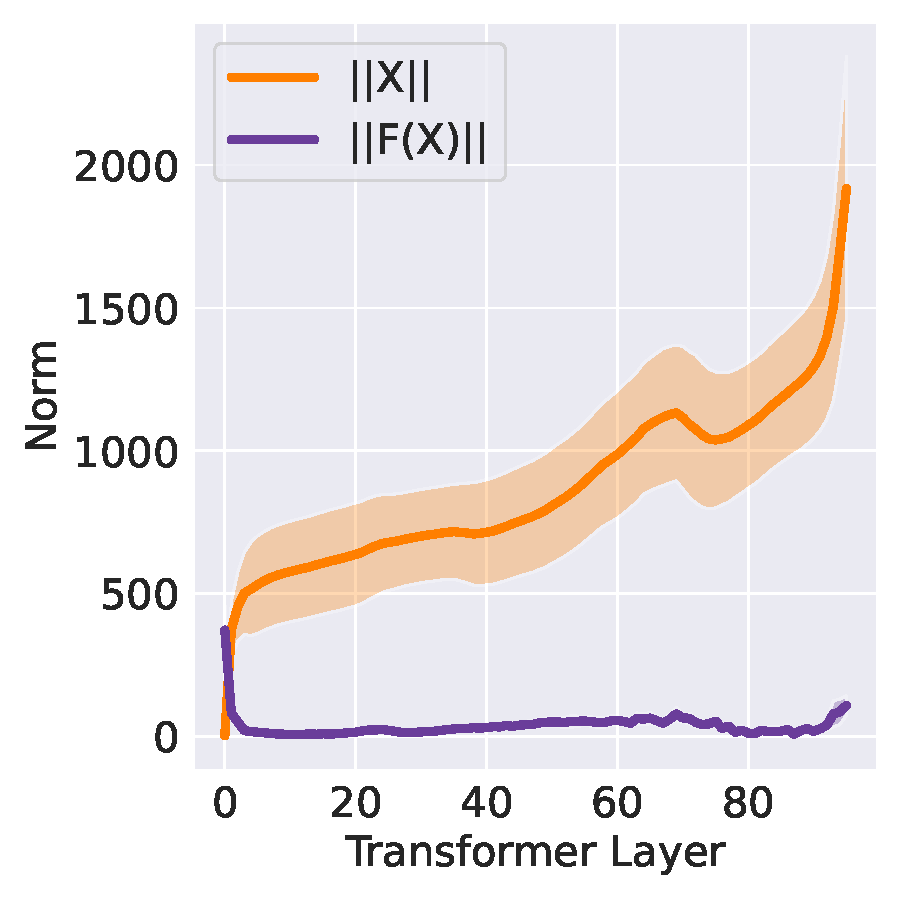
\includegraphics[width=0.22\textwidth]{figure/175b_norm_residual_attention_sqaure.pdf}
    \label{obs:attention_residual}
  } 
    \subfigure[Residual Around MLP]{
    \hspace{1mm}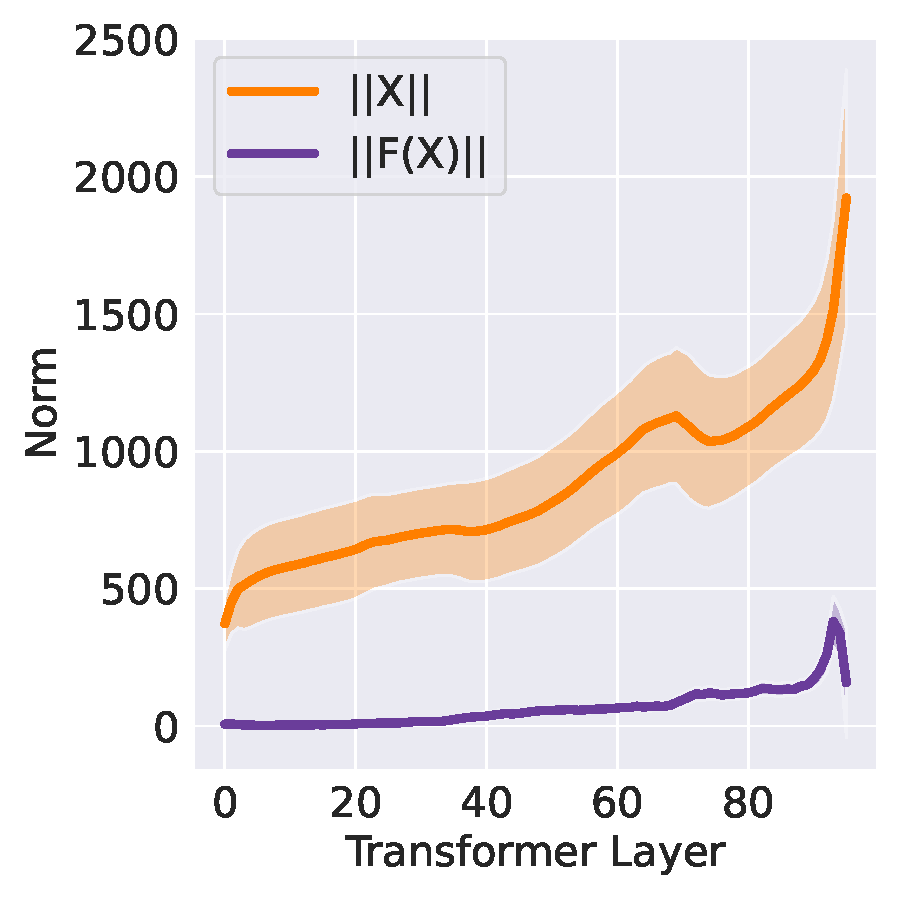
\includegraphics[width=0.22\textwidth]{figure/175b_norm_residual_mlp_sqaure.pdf}
    \label{obs:mlp_residaul}
  } 
  \vspace{-0.3em}
  \caption{\textbf{Slowly Changing Embedding.} Figure (a) shows the median cosine similarity between representations at two consecutive layers across all layers for different OPT models. All models show a similarity greater than 95\%. Figure (b) shows cosine similarity stays high even a few layers apart. For the residual connection $X' = X + F(X)$ inside each block, we plot the $\ell_2$ norm of $X$ and $F(X)$ in Figure (c) and Figure (d). $\|X\|$ is significantly higher than $\|F(X)\|$, which explains the slowly changing embedding.\vspace{-1em}}
  % \caption{ \textbf{Slowly Changing Embedding} We look at the cosine similarity between token embeddings at transformer layer $i$ and transformer layer $i + n$ for the same input.  Figure (a) shows the median cosine similarity between representations at two consecutive layers ($n = 1$) across all layers for different OPT models. All models show a similarity greater than 95\%. Also, similarity increases as the model grow larger. Figure (b), (c), and (d) shows the cosine similarity with various choices of $n$ at every layer. The similarity is near zero at the first layer. Starting at the second layer, cosine similarity remains high and drops a little at later layers. The similarity is lower when $n$ is larger.  \textbf{Residual connection maintains the angle.} There are two residual connections $X' = X + F(X)$ inside each transformer layer, one around the attention block and one around the MLP block. In this figure, we plot the cosine similarity between $X$ and $F(X)$, and the cosine similarity between $X$ and $X'$ in orange color. The similarity between $X'$ and $X$ is extremely high at all layers( except the first layer), while the similarity between $X$ and $F(X)$ is low, almost orthogonal in the majority of layers. To explain this, we plot the $L2$ norm of $X$ and $F(X)$. Except on the first layer, $\|X\|$ is significantly higher than $\|F(X)$. $\|F(X)\|$ is higher at the first layer, which corresponds to the low cosine similarity at the first layer. }
  \label{observation_residual} 
\end{figure}

We first present our observation that embeddings change slowly across consecutive layers. Then we provide a detailed analysis on the phenomenon. Finally, we show its close connection with contextual sparsity.  Details are in Section~\ref{sec:appendix-obs}. 

\textbf{High similar embeddings in consecutive layers:} In Figure~\ref{obs:slowlyevoloving-all}, we show that for the same given input, the cosine similarity between embeddings or activations in two consecutive layers is exceptionally high on 7 different sizes of OPT models. Specifically, we collect activations from each layer while performing OPT model inference on C4 validation set~\cite{2019t5}. Taking OPT-175B as an example, starting from the second layer, the similarity between any two consecutive layers is around 0.99, which indicates that when an input is passed through the model, the direction of its embedding  changes slowly. Interestingly, the most drastic change happens in the first layer. Furthermore, we increase the gap and investigate the similarity between the embedding at layer $l$ and at layer $l + n$ shown in Figure~\ref{obs:slowlyevoloving-175b}. As we increase the gap, the similarity decreases as expected while the differences in cosine similarity between various choices of $n$ are smaller at the shallower layer. We plot the mean similarity, and the standard deviation is indicated by the shading. Similar plots on more models are presented in Appendix~\ref{sec:appendix-obs}.  

\textbf{Connection to residuals:} We verify that the high similarity in embeddings in LLM inference is due to the residual connection. We first dissect the computation graph inside each transformer layer to understand the cause behind this phenomenon. There are two residual connections inside a transformer layer, one around the attention block, and the other one around the MLP block. The residual connection can be written as $X + F(X)$, where $F$ is either the Multi-Head Attention or two MLP Layers.  In Figure~\ref{obs:attention_residual} and Figure~\ref{obs:mlp_residaul},  indeed we can see that $\|X\|$ is significantly greater than $\|F(X)\|$, confirming that embeddings are changing slowly because the residual norm is large.   

\textbf{Connection to Contextual Sparsity:} We take a step deeper trying to understand the reason behind the large residual norm with mathematical modeling.  
We discover that one possible reason for small $\|F(X)\|$ is due to high sparsity. For the MLP Block, high sparsity may contribute to the small norm of $F(X)$ because a large portion of outputs have small norms. Similar reasoning applies to the Attention Block, and thus a large number of attention heads yield small norm outputs.

% uniform attention weights suggest that token embeddings are dissimilar or orthogonal, which can lead to a small norm.

% Figure~\ref{observation:residual} plots the cosine similarity between $X$ and $X + F(X)$, which is close to 1.0, and the cosine similarity between $X$ and $F(X)$, which is close to 0.0. This happens because $\|X\|$ is significantly greater than $\|F(X)\|$, shown in the purple in Figure~\ref{observation:residual}. At the first layer, $\|F(X)\|$ is larger, which explains the low cosine similarity. The magnitude of $L2$ norm is different across models, however, we observe a similar trend with models of different sizes. 

% We further investigate the reason for the small $\|F(X)\|$. Even though there exists a normalization layer before $F(X)$, as shown in Figure~\ref{observation:residual}, layer normalization scale $\|X\|$ to a consistent magnitude across layers (e.g. 85 for OPT-30B, 110 for OPT175B), but not necessarily scale down $\|X\|$. 






% Large language models are typically repetitions of the same architectures. For example, GPT3-175B consists of 96 transformer layers, where each layer is made of an Attention block and an MLP Block. We record the activation after every block and investigate the similarity between these activations in Figure~\ref{obs:slowlyevoloving}. Activation is collected by running OPT models~\cite{} on C4 validation set~\cite{}. We plot the mean similarity and the standard deviation is indicated by the shading. Similar plots on more models are presented in Appendix~\ref{sec:appendix-obs}.

% Our most surprising finding is that the cosine similarity between activations of two consecutive layers is extremely high. Taking OPT175B as an example in Figure~\ref{obs:slowlyevoloving-175b}, the similarity is low, around 0, between the first and the second layer. Starting from the second layer, the similarity between any two consecutive layers is around 0.99 with a small drop to 0.96 toward the ending layers. This indicates that when input data is passed through the model, the direction of its representation vector changes slowly. The exception is the first layer, in which we suspect that token embedding is uniformly mixed with each other, as suggested in~\cite{}.

% Further, we increase the gap and investigate the similarity between the representation at layer $i$ and at layer $i + n$. Generally, as we increase the gap, the similarity decreases as expected. One interesting finding is that the differences in cosine similarity between various choices of $n$ are smaller at the shallower layer. 

% \subsubsection{Empirical Reason}
% % \begin{wrapfigure}{r}{0.15\textwidth}
% %   \begin{center}
% %     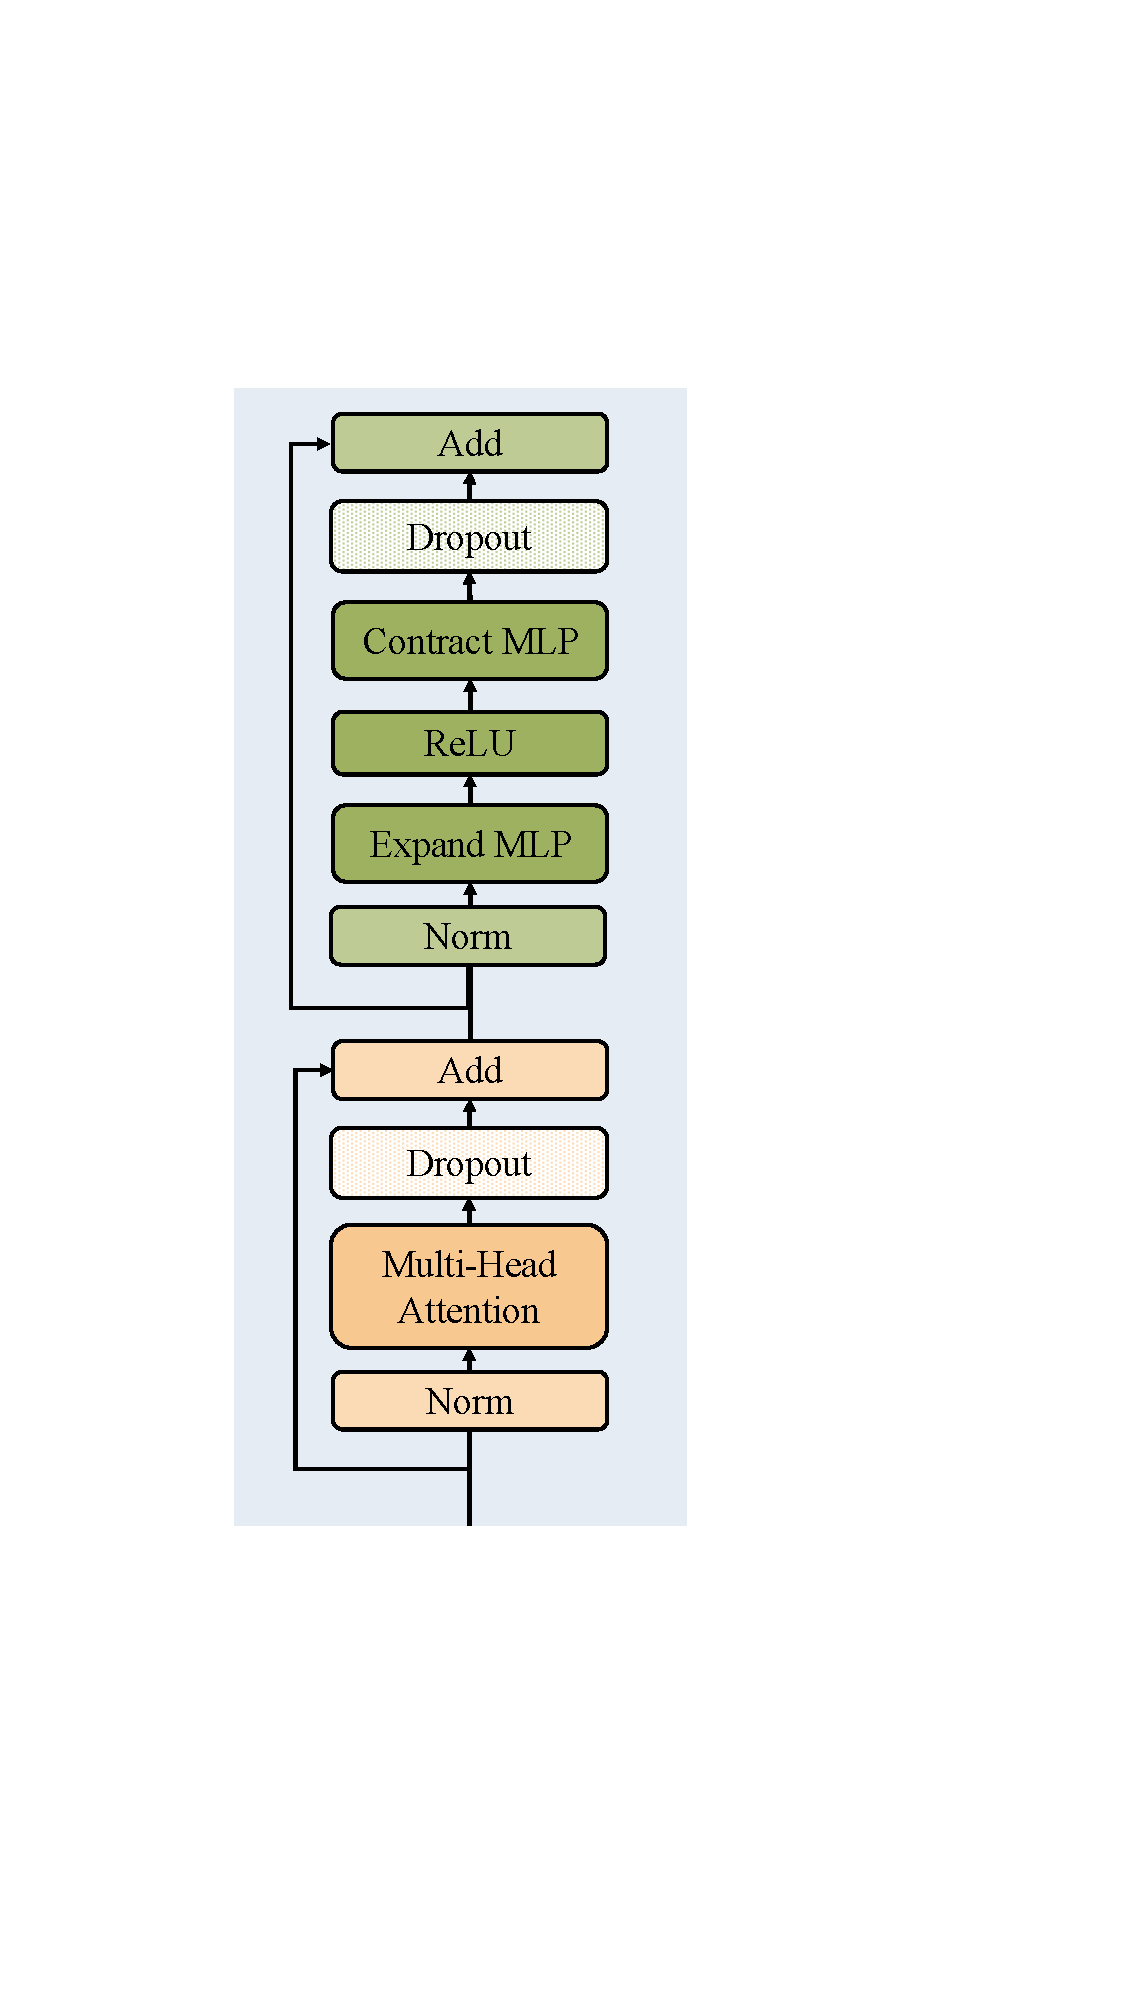
\includegraphics[width=0.15\textwidth]{figure/GPT_Blog_Diagram.pdf}
% %   \end{center}
% %     \label{fig:arch}
% % \end{wrapfigure}
% We dissect the computation graph inside each transformer layer to understand the cause behind this phenomenon. There are two residual connections inside a transformer layer, one around the attention block, and the other one around the MLP block. The residual connection can be written as $X + F(X)$, where $F$ is either the Multi-Head Attention or two MLP Layer, shown in Figure~\ref{fig:arch}. 

% Figure~\ref{observation:residual} plots the cosine similarity between $X$ and $X + F(X)$, which is close to 1.0, and the cosine similarity between $X$ and $F(X)$, which is close to 0.0. This happens because $\|X\|$ is significantly greater than $\|F(X)\|$, shown in the purple in Figure~\ref{observation:residual}. At the first layer, $\|F(X)\|$ is larger, which explains the low cosine similarity. The magnitude of $L2$ norm is different across models, however, the we observe a similar trend with models of different sizes. 


% We further investigate the reason for the small $\|F(X)\|$. Even though there exists a normalization layer before $F(X)$, as shown in Figure~\ref{observation:residual}, layer normalization scale $\|X\|$ to a consistent magnitude across layers (e.g. 85 for OPT-30B, 110 for OPT175B), but not necessarily scale down $\|X\|$.  See Theoretical analysis in Section~\ref{sec:obs_theory}.%??? \Zhao{I will double check this once appendix is finished.}

% High sparsity may also contribute to the small norm of $F(X)$ in the MLP block. We observe high sparsity as a naturally occurring phenomenon in MLP blocks.
% As demonstrated in \cref{observation:sparsity}, we observed that the majority of neurons in the Expand MLP output zero values after the activation function. In the case of OPT-175b, over 95\% of neurons are not activated during inference. 

% \textbf{Theoretical Understanding}
% \label{sec:obs_theory}
% %\textbf{Residual Lower Bound}
% \iffalse
% \begin{lemma}
% Let $\epsilon_1 \in (0,1)$ denote the lower bound of shrinking factor.
%  We denote $x$ as input and denote $y$ as output. We have the residual connection $y = x + F(x)$. For the MLP block $F(x)$,  
%  we have $ \| y - x \|_2 \geq \epsilon_1$. For the attention block $F(x)$,  we have $\| y - x \|_2 \geq \epsilon_1 $.  
% %$ \| x' - x \|_2 \geq \epsilon_1 $
% \end{lemma}
% \fi
%\iffalse
%F(x) is the original MHA, F'(x) is the sparse computation as follows
%\begin{equation*}
%    MHA(x) = [H_1(x), H_2(x)], ...; H_n(x)]W_o
%\end{equation*}
%where $W_o$ is the output projection and $H_n(x)=\vec{0}, H_n(x) \notin S_h$

%F(x) - F'(x) preserve information
%\fi

\textbf{Residual Two Sides Bound:} Besides empirical reasoning, we formally define the computation of LLMs mathematically. Under our computation model, we can show that a shrinking property which is observed by our practical experiments. Proofs are in Appendix \ref{sec:subspace_embedding}, \ref{sec:distances_angles}, \ref{sec:function_approx}.

\begin{lemma}[Informal]
Let $0 < \epsilon_1 < \epsilon_2< 1$ be the lower and upper bound of the shrinking factor.
Let $x$ be the $y$ be the output. We have the residual connection $y = x + F(x)$. For the MLP block $F(x)$,  
 we have $\epsilon_1 \leq \| y - x \|_2 \leq \epsilon_2$. For the attention block $F(x)$,  we have $\epsilon_1 \leq \| y - x \|_2 \leq \epsilon_2 $.  
\end{lemma}






%describe the IO bound, low utilization. What is the latency challenge?



% \begin{figure}[]
%   \centering
%     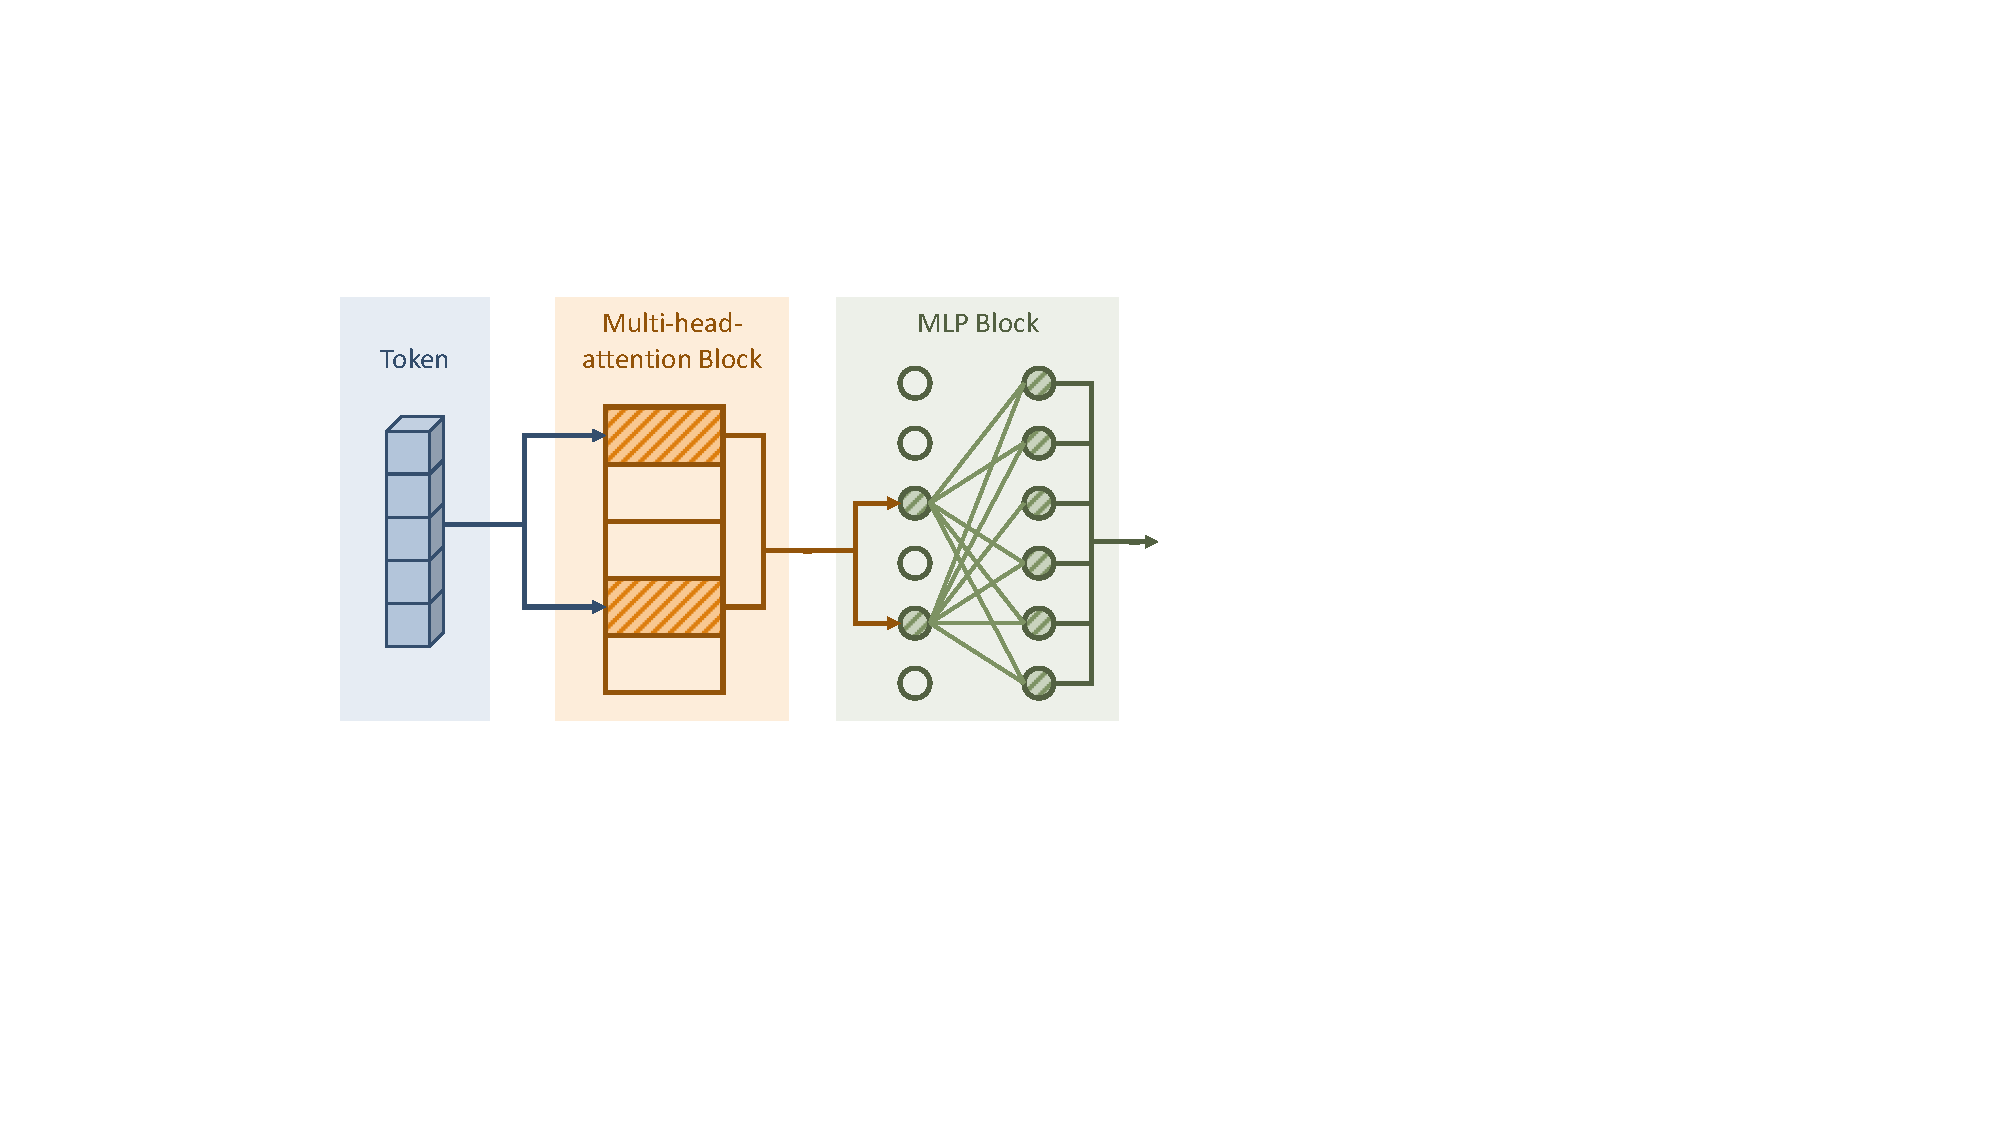
\includegraphics[width=0.5\textwidth]{figure/diagram.pdf}
%   \caption{ \textbf{Sparsified Transformer Layer} }
%   \label{fig:workflow} 
% \end{figure}

%\section{Notations and Basic Definitions}\label{sec:notation_definition}

For a positive integer $n$, let $[ n ] := \{ 1, 2, \cdots, n\}$. For a matrix $A \in \R^{n \times n}$, let $A_{i, :}$ and $A_{:, j}$ be two column vectors corresponding to the $i$-th row and the $j$-th column of $A$ respectively, and $A_{i, j}$ be the entry at the $i$-th row and the $j$-th column. For a vector $x \in \R^n$, let $\sqrt{x} \in \R^{n}$ denote the vector with the $i$-th entry being $\sqrt{x_i}$ and $\diag ( x ) \in \R^{n \times n}$ denote the diagonal matrix with the $i$-th diagonal entry being $x_i$. For two matrices $A, W \in \R^{n \times n}$, let $\| A \|_W := (\sum_{i=1}^n \sum_{j=1}^n W_{i, j} A_{i, j}^2)^{1/2}$ and $W \circ A$ denote the matrix where $(W \circ A)_{i,j} = W_{i,j} A_{i,j}$. For matrix $W \in \R^{n \times n}$, let $D_{W_i} := \diag( W_{i, :} )$ with $i \in [n]$. 

For two vectors $x \in \R^n$ and $w \in \R^n_{\geq 0}$, let $\| x\|_w := (\sum_{i=1}^n w_i x_i^2)^{1/2}$.   For a vector $x$, we denote $\| x \|_2 := ( \sum_{i=1}^n x_i^2 )^{1/2}$ as its $\ell_2$ norm. We denote $\| x \|_p := (\sum_{i=1}^n |x_i|^p)^{1/p}$ as its $\ell_p$ norm. For a square matrix $A$, we denote $\tr[A]$ as the trace of matrix $A$. 

For a matrix $A \in \R^{n \times k}$ (suppose $n \geq k$), we use $\| A \|$ to denote its spectral norm, i.e., $\| A \| = \sup_{x} \| A x \|_2 / \| x \|_2$. We use $\| A \|_F$ to denote its Frobenius norm $\| A \|_F : = (\sum_{i=1}^n \sum_{j=1}^k A_{i,j}^2 )^{1/2}$.

Suppose matrix $A \in \R^{n \times k}$ has SVD decomposition $U \Sigma V^\top$ where $U \in \R^{n \times k}$ (this matrix has orthonormal columns), $\Sigma \in \R^{k \times k}$ is a diagonal matrix, and $V \in \R^{k \times k}$. We call columns of $U$ are singular vectors. We use $A^\dagger \in \R^{k \times n}$ to denote the Moore-Penrose pseudoinverse, then $A^\dagger = V \Sigma^{-1} U^\top$. Suppose $\Sigma \in \R^{k \times k}$ is sorted diagonal matrix, let $\sigma_1, \cdots, \sigma_k$ denote the diagonal entries of $\Sigma$. Then we call $\sigma_i$ the $i$-th singular value of matrix, and we write it as $\sigma_i(A)$.

For any symmetric matrix $B \in \R^{k \times k}$, we define its eigenvalue decomposition as $U \Lambda U^\top$, where $\Lambda$ is a diagonal matrix. Let $\lambda_1, \cdots, \lambda_k$ denote the entries on diagonal of $\Lambda \in \R^{k \times k}$. We say $\lambda_i$ is the $i$-th eigenvalue. Usually we write it as $\lambda_{i}(B)$.

The connection between eigenvalues and singular values is 
\begin{align*}
\sigma_i^2(A) = \lambda_i (A^\top A)
\end{align*}

We use notation $A \succeq 0$ to denote that matrix $A$ is positive semidefinite (psd). Mathematically, $A\succeq 0$ means for all vectors $x$, we have $x^\top A x \geq 0$.

Similarly, for two squarer matrices $A$ and $B$, we use $A \succeq B$ to denote the case where for all vectors $x$, $x^\top  Ax \geq x^\top B x$. 

We use $\Pr[]$ and $\E[]$ for probability and expectation. We denote $\max\{a,b\}$ as the maximum between $a$ and $b$. We denote $\min \{a,b\}$ (resp. $\max\{a,b\}$) as the minimum (reps. maximum) between $a$ and $b$. 

 Throughout, for non-negative real numbers
a and b, we use the notation $a = (1 \pm \epsilon)b ~\text{if}~a \in [(1 - \epsilon)b,(1 + \epsilon)b]$.

\section{Subspace Embeddings and Norm Preserving}\label{sec:subspace_embedding}
In Section \ref{sec:soft_max_func}, we show the norm preserving of the soft-max functions.
In Section \ref{sec:relu_func}, we show the norm preserving of the ReLU function.
In Section \ref{sec:folded_dist}, we introduce the folded Guassian distribution.
In Section \ref{sec:l2_subspace}, we introduce the $\ell_2$ subspace embedding.
In Section \ref{sec:l1_subspace}, we introduce the $\ell_1$ subspace embedding.
In Section \ref{sec:rand_mat}, we introduce different sketching matrices for subspace embedding.

%\iffalse
%Some useful papers here
%\begin{itemize}
%    \item \cite{lwy21}\href{https://arxiv.org/pdf/2104.12946.pdf}{arxiv link}
%    \item \cite{ww18}\href{https://arxiv.org/pdf/1801.04414.pdf}{arxiv link}
%    \item \cite{swz17}\href{https://arxiv.org/pdf/1611.00898.pdf}{arxiv link}
%    \item \cite{w14}\href{https://arxiv.org/pdf/1411.4357.pdf}{arxiv link}
%\end{itemize}
%\fi
%We use $\phi : \R \rightarrow \R$ to denote ReLU function, i.e., $\phi(z) = \max\{z,0\}$.

\subsection{Soft-Max Functions}\label{sec:soft_max_func}


Let $K \in \R^{s \times d}$ and $V \in \R^{d \times s}$.
Inspired by the softmax unit in the attention scheme of large language models. The softmax related regression has been studied in many settings \cite{zhdk23,as23,bsz23,lsz23,dms23,dls23,gms23,lsx+23,gsy23_dp}. In this work, we follow the standard softmax definition. 
We define $\sigma_1 : \R^s \rightarrow \R^s$ to be a softmax function, i.e., for any vector $y \in \R^s$, the $\sigma(y)$ can be written as
\begin{align*}
\sigma_1( y )_i =  \frac{ \exp(y_i) }{ \sum_{j=1}^d \exp(y_j) } , ~~~ \forall i \in [d]
\end{align*}

The standard softmax is $\ell_1$ version. In this work, we also consider the $\ell_2$ generalization. 
We define $\sigma_2: \R^s \rightarrow \R^s$ to be  a softmax function ($\ell_2$ version), i.e., for any vector $y \in \R^s$, the $\sigma(y)$ can be written as
\begin{align*}
\sigma_2( y )_i =  \frac{ \exp( y_i) }{ ( \sum_{j=1}^d \exp(2 y_j) )^{1/2} } , ~~~ \forall i \in [d]
\end{align*}


We define function $f : \R^d \rightarrow \R^d$
\begin{align}\label{eq:f_x}
f (x) =  V \cdot ( \sigma (K \cdot x) ) 
\end{align}

\begin{definition}
We say ${\cal X} \subset \R^d$ is a rank-$k$ subspace, if there is an orthonormal basis $U \in \R^{d \times k}$, for any $x \in {\cal X}$, there is $ y \in \R^k$ such that
\begin{align*}
x = U y.
\end{align*}
\end{definition}

We can have
\begin{lemma}\label{lem:ell_2_subspace_imply_norm_preserve}
Let $\tau \in (0,1)$. Let ${\cal X} \subset \R^d$ denote a subspace with rank $k$.
Let $f$ be defined based on $\sigma_2$ function. 
Let $\ov{V}$ is a random Gaussian matrices with $d \geq \Omega( \epsilon^{-2} ( k + \log(1/\delta) ))$ rows. Let $V = \tau \ov{V} $, then we have with probability $1-\delta$ 
\begin{align*}
(1-\epsilon) \tau \| x \|_2 \leq \| f(x) \| \leq (1+\epsilon) \tau \| x \|_2.
\end{align*}
for all unit vectors $x \in {\cal X}$.

Further, if $d=  O(k + \log(1/\delta))$, then we have
\begin{align*}
0.5 \tau \| x \|_2 \leq \| f(x) \| \leq 2 \tau \| x \|_2.
\end{align*}
\end{lemma} 
\begin{remark}
The above condition implies that $f$ is a shrinking operator but also not shrinking arbitrarily small.
\end{remark}
\begin{proof}
Given $d \geq \Omega( \epsilon^{-2} ( k + \log(1/\delta) ) )$, by using Lemma~\ref{lem:rand_gauss} 
, we have
\begin{align*}
(1-\epsilon)  \| y \|_2 \leq \| \ov{V} y \|_2 \leq (1+\epsilon)  \| y \|_2
\end{align*}
As the input of the function $f$ here is the output of a softmax function ($\ell_2$ version), we know that $\| y \|_2 = 1$.

Thus, we have
\begin{align*}
(1-\epsilon)  \leq \| \ov{V} y \|_2 \leq (1+\epsilon) 
\end{align*} 
By rescaling $V$, we have
\begin{align*}
(1-\epsilon)  \| x \|_2 \leq \| V y \|_2 \leq (1+\epsilon)   \| x \|_2.
\end{align*} 
\end{proof}


\begin{lemma}
Let $\tau \in (0,1)$. Let ${\cal X} \subset \R^d$ denote a subspace with rank $k$. 
Let $f$ be defined based on $\sigma_1$ function. Suppose $\ov{V}$ is a random Gaussian matrix with $d \geq \Omega( (k + \log(1/\delta)) )$ 
rows. Let $V = \frac{1}{2} \tau \ov{V}$.

Then we have
\begin{align*}
\frac{1}{4\sqrt{s}} \tau \cdot \| x \|_2 \leq \| f( x ) \|_2 \leq  \tau \cdot \| x \|_2
\end{align*}
for all unit vectors $x$.
\end{lemma}
\begin{proof}

By property of subspace embedding, we know that if $d \geq \Omega(\epsilon^{-2} (s+\log(1/\delta)))$,
\begin{align*}
(1-\epsilon) \| y \|_2 \leq \| \ov{V} y \|_2 \leq (1+\epsilon) \| y \|_2
\end{align*}
By property of function of $f$, we know we only need to care $\| y \|_1 = 1$, this implies that %\Tianyi{what is reason for the following step?} \Zhao{Because $y$ has length $s$. The following is true forever. You can try some examples. Then you have a feeling why it's true}
\begin{align*}
\frac{1}{\sqrt{s}} \| y \|_1 \leq \| y \|_2 \leq \| y \|_1
\end{align*}

On one hand, we have
\begin{align}\label{eq:vy_upper}
\| \ov{V} y \|_2 \leq &~  (1+\epsilon) \cdot \| y \|_2 \notag\\
\leq &~  (1+\epsilon) \cdot \| y \|_1 \notag\\
=&~  (1+\epsilon),
\end{align}
where the first step follows from $\| \ov{V} y \|_2 \leq (1+\epsilon) \| y \|_2$, the second step follows from $\| y \|_2 \leq \| y \|_1$ and the last step follows from $\| y \|_1  = 1$.

On the other hand, we have
\begin{align}\label{eq:vy_lower}
\| \ov{V} y \|_2 \geq &~ (1-\epsilon) \| y \|_2 \notag\\
\geq &~  \frac{1}{\sqrt{s}} (1-\epsilon) \| y \|_1 \notag\\
=&~ \frac{1}{\sqrt{s}} (1-\epsilon),
\end{align}
where the first step follows from $(1-\epsilon) \| y \|_2 \leq \| \ov{V} y \|_2 $, the second step follows from $\frac{1}{\sqrt{s}} \| y \|_1 \leq \| y \|_2 $ and the last step follows from $\| y \|_1  = 1$.


Combining Eq.~(\ref{eq:vy_lower})%\Tianyi{the equation notation here is weird, should I just delete Eq.}\Zhao{I think ICML template is funny, you can hard code it as what I do}\Tianyi{fixed}
 and Eq.~(\ref{eq:vy_upper}) together, we have
\begin{align*}
(1-\epsilon) \frac{1}{\sqrt{s}}  \leq \| \ov{V} y \|_2 \leq (1+\epsilon) 
\end{align*} 
Choosing $\epsilon = 1/2$, we have %\Tianyi{the following equation should be $  \frac{1}{2\sqrt{s}}  \leq \| \ov{V} y \|_2 \leq  \frac{3}{2}$}
\begin{align*}
 \frac{1}{2\sqrt{s}}  \leq \| \ov{V} y \|_2 \leq 2.
\end{align*}
By $V = \frac{1}{2} \tau \ov{V}$ and $\|x\|_2 = 1$, we have%\Tianyi{the following equation should be  $\frac{1}{4\sqrt{s}} \tau \| x \|_2 \leq \| V y \|_2 \leq   \frac{3}{4}\tau \| x \|_2.$}
\begin{align*}
\frac{1}{4\sqrt{s}} \tau \| x \|_2 \leq \| V y \|_2 \leq   \tau \| x \|_2.
\end{align*} 

\end{proof}

\subsection{ReLU Functions}\label{sec:relu_func}

We use $\phi : \R \rightarrow \R$ to denote ReLU function, i.e., $\phi(z) = \max\{z,0\}$.

We define function $g : \R^d \rightarrow \R^d$
%%%Zhao: Before this label is {eq:f_x}
\begin{align}\label{eq:g_x}
g (x) =  V \cdot ( \phi (K \cdot x) ) 
\end{align}

Let $K \in \R^{s \times d}$ and $V \in \R^{d \times s}$.

\begin{lemma}
%Let $\tau = 2/d$. 
Let ${\cal X} \subset \R^d$ denote a rank-$k$ subspace. %Let $S$ denote a set of points from ${\cal X} \subset \R^d$ sand $|S| \leq n$. 
Let $K$ denote a random Gaussian matrix. Let $V$ denote a random Gaussian matrix. Let $s \geq \Omega( \epsilon^{-2}  k\log(1/ (\delta \epsilon ) ) )$. Let $d \geq \Omega(\epsilon^{-2} (k + \log(1/\delta)))$. Then we know with high probability $1-\delta$, for all unit vector $x \in {\cal X}$
\begin{align*}
(1-\epsilon) \| x \|_2 \leq \| f(x) \|_2 \leq (1+\epsilon) \| x \|_2
\end{align*}
\end{lemma}
\begin{proof}
Suppose $s \geq \Omega( \epsilon^{-2} \log(1/\delta ) )$.


Using Lemma~\ref{lem:lm}, Fact~\ref{fac:key_property_ReLU}, we can show that for each fixed 
\begin{align*}
(1-\epsilon) \| x \|_2 \leq \| \phi(K x ) \|_2 \leq (1+\epsilon) \| x \|_2
\end{align*}
holds with probability $1-\delta$.

By a standard $\epsilon$-net argument (Lemma~\ref{lem:epsilon_net}), the net points in ${\cal X}$ is at most $(10/\epsilon)^{O(k)}$.


Taking a union bound over all the net points, we can show that for all $x \in {\cal X}$
\begin{align*}
(1-\epsilon) \| x \|_2 \leq \| \phi(K x ) \|_2 \leq (1+\epsilon)\| x \|_2
\end{align*}
holds with probability $1-\delta/2$ and $s \geq \Omega( \epsilon^{-2} k \log(1/ (\delta \epsilon) ) )$.

Further, we using Lemma~\ref{lem:rand_gauss}, we can show that
\begin{align*}
(1-\epsilon) \| \phi(K x) \|_2 \leq \| f(x) \|_2 \leq (1+\epsilon) \| \phi(K x) \|_2
\end{align*}
holds with probability $1-\delta/2$.

Combining together,
\begin{align*}
 (1-\epsilon)^2  \| x \|_2 \leq \| f(x) \|_2 \leq (1+\epsilon)^2 \| x \|_2 
\end{align*}
holds with probability $1-\delta$.

Rescaling the $\epsilon$, we complete the proof.

%Choosing $\epsilon = \Theta(1)$, and setting $\alpha = \Theta(\beta)$, we complete the proof.
\end{proof}

\subsection{Folded Gaussian Distribution}\label{sec:folded_dist}

We state a standard tool from literature,
\begin{lemma}[Lemma 1 on page 1325 of Laurent and Massart \cite{lm00}%, Lemma A.7 in \cite{sy21}
]\label{lem:lm}
    Let $X \sim \mathcal{X}_k^2$ be a chi-squared distributed random variable with $k$ degrees of freedom. Each one has zero means and $\sigma^2$ variance. 
    
    Then,
    \begin{align*}
        \Pr[X - k\sigma^2 \geq (2\sqrt{kt} + 2t) \sigma^2]
        \leq & ~ \exp{(-t)}\\
        \Pr[k\sigma^2 - X \geq 2\sqrt{kt}\sigma^2]
        \leq & ~ \exp{(-t)}
    \end{align*}
    Further if $k \geq \Omega(\epsilon^{-2} t)$ and $t \geq \Omega(\log(1/\delta))$, then we have
    \begin{align*}
    \Pr[ | X - k \sigma^2 | \leq \epsilon k \sigma^2 ] \leq \delta.
    \end{align*}
\end{lemma}

We prove the following property,
\begin{fact}\label{fac:key_property_ReLU}
Let $h, q \in \R^p$ be fixed vectors and $h \neq 0, W \in \R^{m \times p}$ be random matrix with i.i.d. entries $W_{i, j} \sim \mathcal{N} (0, \frac{2}{m} )$, and vector $v \in \R^m$ defined as $v_i=\phi ((W h)_i )=\mathbf{1}_{(W(h+q))_i \geq 0}(W h)_i$. Then,
\begin{itemize}
    \item $ |v_i |$ follows i.i.d. from the following distribution: with half probability $ |v_i |=0$, and with the other half probability $ |v_i |$ follows from folded Gaussian distributions $ |\mathcal{N} (0, \frac{2\|h\|^2}{m} ) |$.
    \item $\frac{m\|v\|^2}{2\|h\|^2}$ is in distribution identical to $\chi_\omega^2$ (chi-square distribution of order $\omega$ ) where $\omega$ follows from binomial distribution $\mathcal{B}(m, 1 / 2)$.
\end{itemize}

\end{fact}

\begin{proof}
    We assume each vector $W_i$ is generated by first generating a gaussian vector $g \sim \mathcal{N} (0, \frac{2   I}{m} )$ and then setting $ W_i=\pm g$ where the sign is chosen with half-half probability. Now, $ | \langle W_i, h \rangle |=|\langle g, h\rangle|$ only depends on $g$, and is in distribution identical to $ |\mathcal{N} (0, \frac{2\|h\|^2}{m} ) |$. Next, after the sign is determined, the indicator $\mathbf{1}_{ \langle W_i, h+q \rangle \geq 0}$ is $1$ with half probability and $0$ with another half. Therefore, $ |v_i |$ satisfies the aforementioned distribution. As for $\|v\|^2$, letting $\omega \in\{0,1, \ldots, m\}$ be the variable indicator how many indicators are $1$ , then $\omega \sim \mathcal{B}(m, 1 / 2)$ and $\frac{m\|v\|^2}{2\|h\|^2} \sim \chi_\omega^2$.
\end{proof}
 

\subsection{$\ell_2$ subspace embedding}\label{sec:l2_subspace}

We define a standard notion in sketching technique.\footnote{We remark that sketching technique has widely applied to many applications such as linear regression, low-rank approximation \cite{cw13,nn13,ldfu13,bwz16,c16,rsw16,swz17,swz19}, linear programming \cite{sy21,dly21,jswz21,gs22}, semi-definite programming \cite{gs22,syyz23}, empirical risk minimization\cite{lsz19,qszz23}, training over-parameterized neural network \cite{bpsw21,szz21,als+22,hswz22,z22}.}
\begin{definition}[$\ell_2$ subspace embedding \cite{s06}]\label{def:l2_subspace_embedding}%\cite{w+14}
A $(\epsilon, \delta, \ell_2)$-subspace embedding for the column space of an $n \times d$ matrix $A$ is a matrix $S$ for which %for which all $x \in \R^d$
\begin{align*}
  \Pr [ \forall x \in \mathbb{R}^d,  \|S Ax\|_2^2 = (1 \pm \epsilon) \|Ax\|_2^2 ] \geq 1-\delta.
\end{align*}
%holds with probability $1-\delta$.
The above condition is equivalent to
\begin{align*}
\Pr[ \| U^\top U - U^\top S^\top S U \| \leq \epsilon ] \geq 1-\delta.
\end{align*}
where the $U$ is the orthonormal basis of $A$.
\end{definition}
For the reason of above conditions are equivalent, we refer the readers to the survey \cite{w14}.

We state a standard tool in literature,
\begin{lemma}[Lemma 5 in \cite{w14}]\label{lem:epsilon_net}
Let ${\cal X} \subset\R^d$ be rank $k$. For any $\gamma \in (0,1)$, there is a $\gamma$-net $N$ of ${\cal X}$ for which $|N| \leq (1+4 /\gamma)^k$.
\end{lemma}

\subsection{$\ell_1$ subspace embedding}\label{sec:l1_subspace}

 When $p=1$, using Cauchy random variables, Sohler and Woodruff \cite{sw11} showed there exist $\ell_1$ oblivious subspace embeddings with $O(d \log d)$ rows and $\kappa=O(d \log d)$. This approach was generalized by using $p$-stable random variables in work of Meng and Mahoney \cite{mm13} to $\ell_p$-norms when $1<p<2$, where they showed there exist $\ell_p$ oblivious subspace embeddings with $O(d \log d)$ rows and $\kappa=O ((d \log d)^{1 / p} )$. Unlike the case when $p=2$, due to the large distortion

% Previous impossibility results for dimension reduction in $\ell_1$ \cite{ln04,bc05,cs02} are established by creating a set of $O(n)$ points in $\R^n$ and showing that any (non-oblivious) embedding on them incurs a large distortion. In this paper, we focus on embedding a $d$-dimensional subspace of $\R^n$ into $\R^{\text {poly }(d)}$ using oblivious embeddings. We stress that $O(n)$ points in a $d$-dimensional subspace have a very different structure from $O(n)$ arbitrary points in $\R^n$. Previous results \cite{cp15} showed that any $d$-dimensional subspace in $\R^n$ can be embedded into $\R^{O (d(\log d) \epsilon^{-2} )}$ with $(1+\epsilon)$ distortion in $\ell_1$ using non-oblivious linear embeddings, where $\epsilon>0$ is an arbitrarily small constant. Here the subspace structure is critically used, since Charikar and Sahai \cite{cs02} showed that there exist $O(n)$ points such that any linear embedding $\R^n \rightarrow \R^d$ must incur a distortion of $\Omega(\sqrt{n / d})$, even for non-oblivious linear embeddings.

 In \cite{ww18}, they show for every $1 \leq p<2$, any oblivious subspace embedding with dimension $r$ has distortion $\kappa=\Omega (\frac{1}{ (\frac{1}{d} )^{1 / p} \cdot \log ^{2 / p} r+ (\frac{r}{n} )^{1 / p-1 / 2}} )$. 
 They also give sparse oblivious subspace embeddings for every $1 \leq p<2$ which are optimal in dimension and distortion, up to poly $(\log d)$ factors. Importantly for $p=1$, they achieve $r=O(d \log d), \kappa=O(d \log d)$ and $s=O(\log d)$ non-zero entries per column. 

\begin{definition}[$\ell_1$ subspace embedding]\label{def:l1_subspace_embedding}%\cite{w+14}
Let $0< \alpha < \beta$ be parameters. We will say a matrix $S$ is an $\ell_1$ subspace embedding for an $n \times d$ matrix $A$ if there are constants $c_1, c_2 > 0$ so that for all $x \in \R^{d}$,
\begin{align*}
    \|Ax\|\leq \|SAx\|_1 \leq d^{c_1} \|Ax\|_1,
\end{align*}
and $S$ has at most $d^{c_2}$ rows.
\end{definition}

%\begin{lemma}
%Suppose that $A \in \R^{d \times d}$ is random matrix, and $\|y \|_1=1$, we want to show that
%\begin{align*}
%\| A y \|_1 \approx (1\pm \epsilon) \| y \|_1
%\end{align*}
%\end{lemma}
\subsection{Random Matrices}\label{sec:rand_mat}


\begin{table*}[!ht]
    \centering
\begin{tabular}{|c|l|l|l|}
\hline {\bf Matrices} & $b$ & {\bf Time for} $R \cdot A$ & {\bf Reference} \\
\hline Random Gaussian & $\epsilon^{-2}(d+\log (1 / \delta))$ & $\Tmat(b, n, d)$ & Thm. 6 of \cite{w14} \\
\hline SRHT & $\epsilon^{-2}(\sqrt{d}+\sqrt{\log n})^2 \log (d / \delta)$ & $n d \log  (\epsilon^{-1} d(\log n) )$ & Thm. 7 of \cite{w14} \\
\hline AMS & $\epsilon^{-2}(d+\log (1 / \delta))$ & $\Tmat(b, n, d)$ & Follow from JL guarantee \\
\hline Count-sketch & $\epsilon^{-2} \delta^{-1} d^2$ & $\mathrm{nnz}(A)$ & Thm. 9 of \cite{w14} \\
\hline Sparse embedding & $\epsilon^{-2} d \cdot$ poly $\log (d /(\epsilon \delta))$ & $\epsilon^{-1} \mathrm{nnz}(A)$ poly $\log (d /(\epsilon \delta))$ & Thm. 10 (2) of \cite{w14} \\
\hline Sparse embedding& $\epsilon^{-2} d^{1+\gamma}$ & $\epsilon^{-1} \mathrm{nnz}(A) \operatorname{poly}(1 / \gamma)$ & Thm. 10 (1) of \cite{w14} \\
\hline
\end{tabular}
\caption{Summary for different sketching matrices for subspace embedding. The sketching matrix $R$ has size $b \times n$. The vectors are from the column subspace of matrix $A$ with size $n \times d . \epsilon \in(0,1)$ is the error parameter, and $\delta \in(0,1)$ is the probability parameter. $\mathcal{T}_{\text {mat }}(a, b, c)$ denotes the running time of fast matrix multiplication of two matrices with size $a \times b$ and $b \times c .$ In the first sparse embedding matrix, each column has $s \geq \epsilon^{-1}$ poly $\log (d /(\epsilon \delta))$ non-zero entries;  In the second sparse embedding matrix, each column has $s \geq \epsilon^{-1}$ poly $(1 / \gamma)$ non-zero entries, $\gamma>0$ is a tunable parameter that gives different trade-offs, and $\delta$ can be as small as $1 /$ poly $(d).$ For count-sketch matrices, the subspace embedding guarantee is proved from JL moment property, instead of directly from JL guarantee.}
\label{tab:summary_sketching}
\end{table*}

\begin{lemma}[Theorem 6 of \cite{w14}]\label{lem:rand_gauss}
    Let $0<\epsilon, \delta <1$ and $S=\frac{1}{\sqrt{k}}   R \in \R^{k \times n}$ where the entries $  R_{i, j}$ of $  R$ are independent standard normal random variables. Then if $k=$ $\Theta (\epsilon^{-2}(d+\log (1 / \delta))  )$, then for any fixed $n \times d$ matrix $A$, with probability $1-\delta, S$ is a $(1 \pm \epsilon) \ell_2$-subspace embedding for $A$, that is, simultaneously for all $x \in \R^d, \| S A x\|_2=(1 \pm \epsilon)\|A x\|_2$. Here $C>0$ is an absolute constant.
\end{lemma}


We consider several standard sketching matrices:
\begin{enumerate}
    \item Random Gaussian matrices.
    \item Subsampled randomized Hadamard/Fourier transform (SRHT) matrices \cite{ldfu13}.
    \item AMS sketch matrices \cite{ams96}, random $\{-1,+1\}$ per entry.
    \item Count-Sketch matrices \cite{ccf02}, each column only has one non-zero entry, and is $-1,+1$ half probability each.
    \item Sparse embedding matrices \cite{nn13}, each column only has $s$ non-zero entries, and each entry is $-\frac{1}{\sqrt{s}},+\frac{1}{\sqrt{s}}$ half probability each.
    \item Uniform sampling matrices.
\end{enumerate}

\begin{definition}[Random Gaussian matrix]
    We say $R \in \R^{b \times n}$ is a random Gaussian matrix if all entries are sampled from $\mathcal{N}(0,1 / b)$ independently.
\end{definition}

\begin{definition}[Subsampled randomized Hadamard/Fourier transform matrix \cite{ldfu13}]
    We say $R \in \R^{b \times n}$ is a subsampled randomized Hadamard transform (SRHT) matrix \footnote{ In this case, we require  $\log n$  o be an integer. } if it is of the form $R=\sqrt{n / b} S H D$, where $S \in \R^{b \times n}$ is a random matrix whose rows are b uniform samples (without replacement) from the standard basis of $\R^n, H \in \R^{n \times n}$ is a normalized Walsh-Hadamard matrix, and $D \in \R^{n \times n}$ is a diagonal matrix whose diagonal elements are i.i.d. Rademacher random variables.
\end{definition}

\begin{definition}[AMS sketch matrix \cite{ams96}]
   Let $h_1, h_2, \cdots, h_b$ be $b$ random hash functions picking from a 4-wise independent hash family $\mathcal{H}=\{h:[n] \rightarrow\{-\frac{1}{\sqrt{b}},+\frac{1}{\sqrt{b}}\}\}$. Then $R \in \R^{b \times n}$ is a AMS sketch matrix if we set $R_{i, j}=h_i(j)$
\end{definition}

\begin{definition}[Count-sketch matrix \cite{ccf02}]
    Let $h:[n] \rightarrow[b]$ be a random 2-wise independent hash function and $\sigma:[n] \rightarrow\{-1,+1\}$ be a random 4-wise independent hash function. Then $R \in \R^{b \times n}$ is a count-sketch matrix if we set $R_{h(i), i}=\sigma(i)$ for all $i \in[n]$ and other entries to zero.
\end{definition}

\begin{definition}[Sparse embedding matrix I \cite{nn13}]
    We say $R \in \R^{b \times n}$ is a sparse embedding matrix with parameter $s$ if each column has exactly $s$ non-zero elements being $\pm 1 / \sqrt{s}$ uniformly at random, whose locations are picked uniformly at random without replacement (and independent across columns) \footnote{For our purposes the signs need only be $O(\log d)$-wise independent, and each column can be specified by a $O(\log d)$-wise independent permutation, and the seeds specifying the permutations in different columns need only be $O(\log d)$-wise independent.}.
\end{definition}

\begin{definition}[Sparse embedding matrix II \cite{nn13}]
   Let $h:[n] \times[s] \rightarrow[b / s]$ be a random 2-wise independent hash function and $\sigma:[n] \times[s] \rightarrow\{-1,1\}$ be a 4-wise independent. Then $R \in \R^{b \times n}$ is a sparse embedding matrix II with parameter $s$ if we set $R_{(j-1) b / s+h(i, j), i}=\sigma(i, j) / \sqrt{s}$ for all $(i, j) \in[n] \times[s]$ and all other entries to zero \footnote{This definition has the same behavior as sparse embedding matrix I for our purpose}.
\end{definition}

\begin{definition}[Uniform sampling matrix]
    We say $R \in \R^{b \times n}$ is a uniform sampling matrix if it is of the form $R=\sqrt{n / b} S D$, where $S \in \R^{b \times n}$ is a random matrix whose rows are b uniform samples (without replacement) from the standard basis of $\R^n$, and $D \in \R^{n \times n}$ is a diagonal matrix whose diagonal elements are i.i.d. Rademacher random variables.
\end{definition}



%The above is only one layer, do we need multiple layer.
\section{Distances, Angles, and Inner Product}\label{sec:distances_angles}

Most of the properties in this section are very standard in literature, e.g., see \cite{gsyz23}.

Let $U \in \R^{n \times k}$ denote an orthonormal basis, we use $U_{\bot} \in \R^{n \times (n-k)}$ denote the matrix such that $U U^\top + U_{\bot} U_{\bot}^\top = I_n$.


\begin{definition}\label{def:angle_and_distance}
Let $X \in \R^{n \times k}$ and $Y \in \R^{n \times k}$.

For any matrix $X$, and for orthogonal matrix $Y$ ($Y^\top Y = I_k$) we define
%\Tianyi{what is the definition of $A_\bot$} \Zhao{See above}
\begin{itemize}
    \item $\tan \theta(Y,X) := \| Y_{\bot}^\top X ( Y^\top X )^{-1} \|$
\end{itemize}
For orthogonal matrices $Y$ and $X$ ($Y^\top Y = I_k$ and $X^\top X = I_k$), we define %\Tianyi{what is $\sigma$} \Zhao{Read notation section}
\begin{itemize}
    \item $\cos \theta (Y,X) := \sigma_{\min} (Y^\top X)$. 
    \begin{itemize} 
        \item It is obvious that $\cos (Y,X) = 1/ \| (Y^\top X)^{-1} \|$ and $\cos(Y,X) \leq 1$.
    \end{itemize}
    \item $\sin \theta(Y,X) := \| (I - Y Y^\top) X \|$.
    \begin{itemize} 
        \item It is obvious that $\sin \theta(Y,X) = \| Y_{\bot} Y_{\bot}^\top X \| = \| Y_{\bot}^\top X \|$ and $\sin \theta(Y,X) \leq 1$.
    \end{itemize}
    \item $\dist(Y,X) := \min_{Q \in O_k} \| YQ - X \|$
\end{itemize}  
where $O_k$ is the set of $k \times k$ orthogonal matrices. 
\end{definition}

\begin{lemma}[Structural lemma for orthogonal matrices]
\label{lem:trig_structural}
Let $X, Y\in \R^{n\times k}$ be orthogonal matrices. Then
\begin{align*}
    (Y^\top X)_\bot = & ~ Y_\bot^\top X.
\end{align*}
\end{lemma}

\begin{proof}
    Let us first compute the Gram of $Y^\top X$, which is
\begin{align*}
    X^\top YY^\top X 
    = & ~ X^\top (I-Y_\bot Y_\bot^\top) X \\
    = & ~ X^\top X-X^\top Y_\bot Y_\bot^\top X \\
    = & ~ I_k-X^\top Y_\bot Y_\bot^\top X,
\end{align*}
where the first step follows from $Y_\bot Y_\bot^\top + YY^\top = I$, the second step follows from simple algebra, and the last step follows from $X$ is an orthogonal matrix, so $X^\top = X^{-1}$.

This means that $(Y^\top X)_\bot=Y_\bot^\top X$.
\end{proof}

\begin{lemma}[Orthogonal and inverse share singular vectors]
\label{lem:perp_inv_singular}
Let $A\in \R^{k\times k}$ be non-singular, then $A_\bot$ and $A^{-1}$ have the same set of singular vectors. Consequently, $\|A_\bot A^{-1}\|=\|A_\bot\|\|A^{-1}\|$. 

\end{lemma}

\begin{proof}
     Let $A\in \R^{k\times k}$ and $A^\top A+A_\bot^\top A_\bot=I_k$, we will show that $\|A_\bot A^{-1}\|=\|A_\bot \| \|A^{-1}\|$. Let $x\in \R^k$ be the unit eigenvector of $A$ that realizes the spectral norm, note that
\begin{align*}
    \|A_\bot x\|_2^2 = & ~ 1-\|A\|^2,
\end{align*}
we argue that $x$ corresponds to the smallest singular value of $A_\bot$ via contradiction. Suppose there exists some unit vector $y$ with $\|A_\bot y\|_2 < \|A_\bot x\|_2$, by definition, we know that $\|A_\bot y\|_2^2+\|Ay\|_2^2=1$, this means that $\|Ay\|_2>\|Ax\|_2=\|A\|$, contradicts the definition of spectral norm. Similarly, if $z$ is the unit vector that realizes the spectral norm of $A_\bot$, then it is also singular vector corresponds to the smallest singular value of $A$, or equivalently, the spectral norm of $A^{-1}$. Our above argument essentially implies that $A_\bot$ and $A^{-1}$ have the same set of singular vectors. The proof is then straightforward: suppose $A_\bot z=\lambda z$ and $A^{-1}z=\mu z$, then
\begin{align*}
    A_\bot A^{-1} z 
    = & ~ A_\bot \mu z \\
    = & ~ \mu (A_\bot z) \\
    = & ~ \lambda \mu z,
\end{align*}
where the first step follows from our assumption, the second step follows from $\mu$ is a real number and a real number multiplying a matrix is commutative and follows from the associative property, and the third step follows from our assumption.

Thus, we have $\|A_\bot A^{-1}\|=\|A_\bot\|\|A^{-1}\|$, and we have proved the assertion.
\end{proof}

\begin{lemma}\label{lem:tan_is_sin_cos}
Let $X, Y\in \R^{n\times k}$ be orthogonal matrices, then 
\begin{align*}
    \tan \theta(Y,X) = & ~ \frac{\sin \theta(Y,X)}{\cos \theta(Y,X)}.
\end{align*}
\end{lemma}


\begin{proof}
Due to Lemma~\ref{lem:trig_structural}, we have $(Y^\top X)_\bot=Y^\top_\bot X$. Thus, $\tan\theta(Y,X)=\|(Y^\top X)_\bot (Y^\top X)^{-1}\|$. The proof then follows straightforwardly from Lemma~\ref{lem:perp_inv_singular}.
\end{proof}

\begin{lemma}\label{lem:sin^2_and_cos^2_is_1}
Let $X, Y\in \R^{n\times k}$ be orthogonal matrices, then $\sin^2\theta(Y, X) + \cos^2\theta(Y,X) =1$.
\end{lemma}
\begin{proof}
Recall that $\cos\theta(Y,X)=\frac{1}{\|(Y^\top X)^{-1}\|}$ and $\sin\theta(Y,X)=\|Y_\bot^\top X\|$, by Lemma~\ref{lem:trig_structural}, we know that $(Y^\top X)_\bot=Y^\top_\bot X$, therefore $\sin\theta(Y,X)=\|(Y^\top X)_\bot \|$. Let $A:=Y^\top X$, by Lemma~\ref{lem:perp_inv_singular}, we know that $A_\bot$ and $A^{-1}$ have the same singular vectors, or equivalently, the singular vector realizing $\|A_\bot\|$ corresponds to the smallest singular value of $A$. Let $z\in \R^k$ be the unit singular vector with singular value $\|A_\bot\|$, then
\begin{align*}
    z^\top A^\top Az+z^\top A_\bot^\top A_\bot z = & ~ 1, \\
    \|A_\bot\|^2+\sigma_{\min}^2(A) = & ~ 1, \\
    \cos^2\theta(Y,X)+\sin^2\theta(Y,X) = & ~ 1.
\end{align*}
This completes the proof.
\end{proof}


\subsection{Angle is close}

\begin{lemma}
Let $\epsilon \in (0,0.1)$
Let $x$ denote a unit vector, i.e., $\| x \|_2 = 1$.

Let $z = (x+y) / \| x + y\|_2$.

If $ \| y \|_2 \leq \epsilon \cdot \| x \|_2$, then
\begin{align*}
\sqrt{1-\langle x, z \rangle^2} \leq 2 \sqrt{\epsilon} 
\end{align*}
\end{lemma}
\begin{proof}
We have
\begin{align*}
 \| x + y \|_2 
 \geq & ~\| x \|_2 - \| y \|_2 \\
\geq & ~ 1- \epsilon
\end{align*}
where the first step follows from triangle inequality.

We also have
\begin{align}\label{eq:x_y_bound}
 \| x + y \|_2 
 \leq & ~\| x \|_2 + \| y \|_2 \notag \\
\leq & ~ 1 + \epsilon
\end{align}


We have
\begin{align}\label{eq:1_minus_eps}
(1- \epsilon)^2 \geq 1- 2\epsilon
\end{align}

We also have
\begin{align}\label{eq:1_plus_eps}
\frac{1}{(1+\epsilon)^2} \geq 1- 3 \epsilon
\end{align}
where $\epsilon \in (0,0.1)$.



Combining Eq.~(\ref{eq:1_minus_eps}) and Eq.~(\ref{eq:1_plus_eps}), we have
\begin{align}\label{eq:1_2eps}
\frac{1}{(1+\epsilon)^2} \cdot ( 1 - \epsilon )^2 \geq &~ (1-2\epsilon) \cdot (1-3 \epsilon) \notag\\
=&~ 1 -5 \epsilon + 6 \epsilon^2 \notag\\
\geq &~  1 - 5\epsilon + \epsilon \notag\\
=&~ 1 - 4 \epsilon 
\end{align}
where the first step follows from Eq.~(\ref{eq:1_minus_eps}) and Eq.~(\ref{eq:1_plus_eps}) and the rest of them follow from simple algebra.


Finally, we have
\begin{align*}
1 - \langle x, z \rangle^2
= & ~ 1 - \langle x, \frac{x+y}{ \| x + y \|_2 } \rangle^2 \\
= & ~ 1 - \frac{1}{\| x + y \|_2^2} \langle x , x+y \rangle^2 \\
= & ~ 1 - \frac{1}{\| x + y \|_2^2} \cdot ( \| x \|_2^2 + \langle x , y \rangle )^2 \\
= & ~  1 - \frac{1}{\| x + y \|_2^2} \cdot ( 1 + \langle x , y \rangle )^2 \\
\leq & ~ 1 - \frac{1}{(1+\epsilon)^2} \cdot ( 1 + \langle x , y \rangle )^2 \\
\leq & ~ 1 - \frac{1}{(1+\epsilon)^2} \cdot ( 1 - \epsilon )^2 \\
\leq & ~ 1 -  (1- 4 \epsilon) \\
= & ~ 4 \epsilon,
\end{align*}
where the first step follow the definition of $z$, the second step follows from the reorganization, the third step follows from the definition of inner product, the fourth step follows from $\| x \|_2 = 1$, the fifth step follows from Eq.~(\ref{eq:x_y_bound}), the sixth step follows from  $1+\langle x,y\rangle \geq 1 - | \langle x , y \rangle | \geq 1 - \| x \|_2 \cdot \| y \|_2 \geq 1- \epsilon$, the seventh step follows from Eq.~(\ref{eq:1_2eps}) and the last step follows from simple algebra.


\end{proof}
%Check if $\| f(x) + x \|_2 \approx(1 \pm \epsilon) \| x \|_2$, then cosin is good.

\section{Function Approximations}\label{sec:function_approx}

% \Zhao{Write a roadmap}
We first we show the function approximation for two operators in Section \ref{sec:fun_app_app}, which means that there are two functions. Then we show the function approximations for four operators in Section \ref{sec:fun_app_operators_app}.


\subsection{Function Approximations for Two Operators}\label{sec:fun_app_app}

\begin{lemma}
Let $f_1 : \R^d \rightarrow \R^d$ and let $f_2 : \R^d \rightarrow \R^d$.

Assume the the following conditions
\begin{itemize}
    \item Condition 1a. $f_1$ is a linear function 
    \item Condition 1b. $\| f_1(x) \|_2 \leq \epsilon_1 \| x \|_2$ ($f_1$ is shrinking)
    \item Condition 1c. $\| f_1 (x)  -f_1(y) \|_2 \leq L_1 \| x - y \|_2$ ($f_1$ is Lipschitz)
    \item Condition 2a. $f_2$ is a linear function 
    \item Condition 2b. $\| f_2(x) \|_2 \leq \epsilon_2 \| x \|_2$  ($f_2$ is shrinking)
    \item Condition 2c. $\| f_2 (x)  -f_2(y) \|_2 \leq L_2 \| x - y \|_2$ ($f_2$ is Lipschitz)
\end{itemize}

We define three functions
\begin{itemize}
\item 
\begin{align*}
g_1 (x) = : & ~ (I + f_1) \cdot (I + f_2) (x)  \\
= & ~ x + f_2(x) + f_1 ( x + f_2(x) )
\end{align*}
\item
\begin{align*}
g_2 (x) = : & ~ (I + f_2) \cdot (I + f_1) (x)  \\
= & ~ x + f_1(x) + f_2 ( x + f_1(x) )
\end{align*}
\item
\begin{align*}
g_3 (x) = : & ~ (I + f_1 + f_2) (x)  \\
= & ~ x + f_1(x) + f_2(x)
\end{align*}
\end{itemize}
Then we can show that
\begin{itemize}
    \item Part 1. $\| g_1 (x) - g_2 (x) \|_2 \leq 2 \epsilon_1 \epsilon_2 \| x \|_2$(if $f_1$ and $f_2$ are linear functions)
    \item Part 2. $\| g_1 (x) - g_2 (x) \|_2 \leq (\epsilon_2 \cdot L_1+ \epsilon_1 \cdot L_2) \| x \|_2  $  (if $f_1$ and $f_2$ are Lipschitz functions)
    \item Part 3. $\| g_1 (x) -g_3 (x) \|_2 \leq \epsilon_1 \epsilon_2 \| x \|_2$ (if $f_1$ is a linear function)
    \item Part 4. $\| g_1 (x) -g_3 (x) \|_2 \leq \epsilon_2 \cdot L_1 \| x \|_2$ (if $f_1$ is a Lipschitz function)
    \item Part 5.  $\| g_2 (x) -g_3 (x) \|_2 \leq \epsilon_1 \epsilon_2 \| x \|_2$ (if $f_2$ is a linear function)
    \item Part 6. $\| g_2 (x) -g_3 (x) \|_2 \leq \epsilon_1 \cdot L_2 \| x \|_2$ (if $f_2$ is a Lipschitz function)
\end{itemize}
\end{lemma}
\begin{proof}

{\bf Part 1.}



We have 
\begin{align*}
\| g_1 (x) - g_2 (x) \|_2 \leq &~ \|g_1(x) - g_3(x) \|_2 + \|g_3(x) - g_2(x)\|_2\\
\leq &~   \epsilon_1 \epsilon_2 \| x \|_2 + \epsilon_1 \epsilon_2 \| x \|_2 \\
= &~  2 \epsilon_1 \epsilon_2 \| x \|_2
\end{align*}
where the first step follows from triangular inequality, the second step follows from Part 3 and Part 5 and the last step follows from simple algebra.

{\bf Part 2.}

We have 
\begin{align*}
\| g_1 (x) - g_2 (x) \|_2 \leq &~ \|g_1(x) - g_3(x) \|_2 + \|g_3(x) - g_2(x)\|_2\\
\leq &~  \epsilon_2 \cdot L_1 \| x \|_2+ \epsilon_1 \cdot L_2 \| x \|_2 \\
= &~  (\epsilon_2 \cdot L_1+ \epsilon_1 \cdot L_2) \| x \|_2 
\end{align*}
where the first step follows from triangular inequality, the second step follows from Part 4 and Part 6 and the last step follows from simple algebra.



{\bf Part 3.}

We have 
\begin{align*}
\| g_1 (x) - g_3(x) \|_2
= & ~ \| f_1(x+ f_2(x) ) - f_1(x) \|_2 \\
= & ~ \| f_1 (x+ f_2(x) - x) \|_2 \\
= & ~ \| f_1 (f_2(x) ) \|_2 \\
\leq & ~ \epsilon_1 \cdot \| f_2(x) \|_2 \\
\leq & ~ \epsilon_1 \cdot \epsilon_2 \cdot \| x \|_2,
\end{align*}
where the first step follows from the definition of $g_1$ and $g_3$, the second step follows from the fact that $f_1$ is a linear function, the third step follows from simple algebra, the fourth step follows from Condition 1b and the last step follows from Condition 2b.

{\bf Part 4.}

\begin{align*}
\| g_1 (x) - g_3(x) \|_2
= & ~ \| f_1(x+ f_2(x) ) - f_1(x) \|_2 \\
\leq & ~L_1 \cdot \| x+ f_2(x) - x \|_2  \\
= & ~  L_1 \cdot \| f_2 (x) \|_2 \\
\leq & ~ L_1 \cdot \epsilon_2 \| x \|_2,
\end{align*}
where the first step follows from definition of $g_1$ and $g_3$, the second step follows from Condition 1c, the third step follows from simple algebra and the last step follows from Condition 2b. 
\end{proof}

{\bf Part 5.}

We have 
\begin{align*}
\| g_2 (x) - g_3(x) \|_2
= & ~ \| f_2(x+ f_1(x) ) - f_2(x) \|_2 \\
= & ~ \| f_2 (x+ f_1(x) - x) \|_2 \\
= & ~ \| f_2 (f_1(x) ) \|_2 \\
\leq & ~ \epsilon_2 \cdot \| f_1(x) \|_2 \\
\leq & ~ \epsilon_2 \cdot \epsilon_1 \cdot \| x \|_2,
\end{align*}
where the first step follows from the definition of $g_2$ and $g_3$, the second step follows from the fact that $f_2$ is a linear function, the third step follows from simple algebra, the fourth step follows from Condition 2b and the last step follows from Condition 1b.

{\bf Part 6.}

\begin{align*}
\| g_2 (x) - g_3(x) \|_2
= & ~ \| f_2(x+ f_1(x) ) - f_2(x) \|_2 \\
\leq & ~L_2 \cdot \| x+ f_1(x) - x \|_2  \\
= & ~  L_2 \cdot \| f_1 (x) \|_2 \\
\leq & ~ L_2 \cdot \epsilon_1 \| x \|_2,
\end{align*}
where the first step follows from definition of $g_1$ and $g_3$, the second step follows from Condition 2c, the third step follows from simple algebra and the last step follows from Condition 1b. 

\subsection{Function Approximations for Four Operators}\label{sec:fun_app_operators_app}

\begin{lemma}
For each $i \in [4]$, we assume the following conditions
\begin{itemize}
    \item i(a) $f_i$ is a linear function
    \item i(b) $\| f_i(x) \|_2 \leq \epsilon_i \| x \|_2$ ($f_i$ is shriking)
    \item i(c)  $\| f_i(x) - f_i(y) \|_2 \leq L_i \| x-y\|_2$ ($f_i$ is Lipschitz)
\end{itemize}
We define three functions
\begin{itemize}
    \item $g_1(x):= (I+ f_1) \cdot (I + f_2) \cdot (I + f_3) \cdot (I + f_4) (x)$
    \item $g_2(x): = (I+ f_1) \cdot (I + f_3) \cdot (I + f_2) \cdot (I + f_4) (x)$
    \item $g_3(x) := (I + f_1 + f_2 + f_3 + f_4) (x)$
\end{itemize}
Then, we can show that
\begin{itemize}
    \item Part 1. $\| g_1 (x) - g_2 (x ) \|_2 \leq 2 ( \epsilon_1 \epsilon_2+ \epsilon_1 \epsilon_3 + \epsilon_1 \epsilon_4
        +\epsilon_2\epsilon_3+ \epsilon_2 \epsilon_4
        +\epsilon_3 \epsilon_4 
         + \epsilon_1 \epsilon_2 \epsilon_3 + \epsilon_1 \epsilon_2 \epsilon_4 + \epsilon_1 \epsilon_3 \epsilon_4 +\epsilon_2 \epsilon_3 \epsilon_4 + \epsilon_1 \epsilon_2 \epsilon_3 \epsilon_4) \|x\|_2$ (if $f_i,~\forall i \in [4]$ are linear functions)
    \item Part 2. $\| g_1 (x) - g_2 (x ) \|_2  \leq (2L_1 \epsilon_2  + 2L_1 \epsilon_3  +2L_1 \epsilon_4   +
        L_2 \epsilon_3  + 2L_2  \epsilon_4  + 2L_3  \epsilon_4  +
        2L_1 \epsilon_2 \epsilon_3  +2L_1 \epsilon_2 \epsilon_4   +2L_1 \epsilon_3 \epsilon_4 +
         L_2 \epsilon_3 \epsilon_4  +
        2L_1 \epsilon_2 \epsilon_3 \epsilon_4 + 
         L_3 \epsilon_2 +
          L_3 \epsilon_2 \epsilon_4) \| x\|_2$ (if $f_i,~\forall i \in [4]$ are Lipschitz functions)
    \item Part 3. $\| g_1 (x) - g_3 (x ) \|_2 \leq ( \epsilon_1 \epsilon_2+ \epsilon_1 \epsilon_3 + \epsilon_1 \epsilon_4
        +\epsilon_2\epsilon_3+ \epsilon_2 \epsilon_4
        +\epsilon_3 \epsilon_4 
         + \epsilon_1 \epsilon_2 \epsilon_3 + \epsilon_1 \epsilon_2 \epsilon_4 + \epsilon_1 \epsilon_3 \epsilon_4 +\epsilon_2 \epsilon_3 \epsilon_4 + \epsilon_1 \epsilon_2 \epsilon_3 \epsilon_4) \|x\|_2$ (if $f_i,~\forall i \in [4]$ are linear functions)
    \item Part 4. $\| g_1 (x) - g_3 (x ) \|_2 \leq (L_1 \epsilon_2  + L_1 \epsilon_3  +L_1 \epsilon_4   +
        L_2 \epsilon_3  + L_2  \epsilon_4  + L_3  \epsilon_4  +
        L_1 \epsilon_2 \epsilon_3  +L_1 \epsilon_2 \epsilon_4   +L_1 \epsilon_3 \epsilon_4 +
        L_2 \epsilon_3 \epsilon_4  +
        L_1 \epsilon_2 \epsilon_3 \epsilon_4)  \|x \|_2   $ (if $f_i,~\forall i \in [4]$ are Lipschitz functions)
    \item Part 5. $\| g_2 (x) - g_3 (x ) \|_2\leq ( \epsilon_1 \epsilon_2+ \epsilon_1 \epsilon_3 + \epsilon_1 \epsilon_4
        +\epsilon_2\epsilon_3+ \epsilon_2 \epsilon_4
        +\epsilon_3 \epsilon_4 
         + \epsilon_1 \epsilon_2 \epsilon_3 + \epsilon_1 \epsilon_2 \epsilon_4 + \epsilon_1 \epsilon_3 \epsilon_4 +\epsilon_2 \epsilon_3 \epsilon_4 + \epsilon_1 \epsilon_2 \epsilon_3 \epsilon_4) \|x\|_2$ (if $f_i,~\forall i \in [4]$ are linear functions)
    \item Part 6.$\| g_2 (x) - g_3 (x ) \|_2\leq  (L_1 \epsilon_2 + L_1 \epsilon_3 + L_1 \epsilon_4 +
        L_2 \epsilon_4+
        L_3 \epsilon_2 + L_3 \epsilon_4+
        L_1 \epsilon_2 \epsilon_3 + L_1 \epsilon_2 \epsilon_4 + L_1 \epsilon_3 \epsilon_4+
        L_3 \epsilon_2 \epsilon_4+
        L_1  \epsilon_2 \epsilon_3 \epsilon_4) \| x\|_2\\$ (if $f_i,~\forall i \in [4]$ are Lipschitz functions)
\end{itemize}
\end{lemma}
\begin{proof}

{\bf Part 1.}

We have 
\begin{align*}
\| g_1 (x) - g_2 (x) \|_2 \leq &~ \|g_1(x) - g_3(x) \|_2 + \|g_3(x) - g_2(x)\|_2\\
\leq &~   2 ( \epsilon_1 \epsilon_2+ \epsilon_1 \epsilon_3 + \epsilon_1 \epsilon_4
        +\epsilon_2\epsilon_3+ \epsilon_2 \epsilon_4
        +\epsilon_3 \epsilon_4 
         + \epsilon_1 \epsilon_2 \epsilon_3 + \epsilon_1 \epsilon_2 \epsilon_4 + \epsilon_1 \epsilon_3 \epsilon_4 +\epsilon_2 \epsilon_3 \epsilon_4 + \epsilon_1 \epsilon_2 \epsilon_3 \epsilon_4) \|x\|_2
\end{align*}
where the first step follows from triangular inequality and the last step follows from Part 3 and Part 5.

{\bf Part 2.}

We have 
\begin{align*}
\| g_1 (x) - g_2 (x) \|_2 \leq &~ \|g_1(x) - g_3(x) \|_2 + \|g_3(x) - g_2(x)\|_2\\
\leq &~    (2L_1 \epsilon_2  + 2L_1 \epsilon_3  +2L_1 \epsilon_4   +
        L_2 \epsilon_3  + 2L_2  \epsilon_4  + 2L_3  \epsilon_4  +
        2L_1 \epsilon_2 \epsilon_3  +2L_1 \epsilon_2 \epsilon_4   +2L_1 \epsilon_3 \epsilon_4 +\\
        &~ L_2 \epsilon_3 \epsilon_4  +
        2L_1 \epsilon_2 \epsilon_3 \epsilon_4 + 
         L_3 \epsilon_2 +
          L_3 \epsilon_2 \epsilon_4) \| x\|_2
\end{align*}
where the first step follows from triangular inequality and the last step follows from Part 4 and Part 6.



    {\bf  Part 3.}
    We have
    \begin{align*}
       \| g_1 (x) - g_3 (x ) \|_2 =  &~ \| (I+ f_1) \cdot (I + f_2) \cdot (I + f_3) \cdot  (x + f_4(x) ) - (I + f_1 + f_2 + f_3 + f_4) (x) )  \|_2 \\
        =  &~ \| (x + f_4(x)  + f_3(x + f_4(x)) + f_2(x + f_4(x)  +\\
        &~ f_3(x + f_4(x)))+ f_1(x + f_4(x)  + f_3(x + f_4(x) ) + f_2(x + f_4(x)  + f_3(x + f_4(x) )))  \\
        &~ - (I + f_1 + f_2 + f_3 + f_4) (x) )  )  \|_2 \\
        =  &~ \|    f_3( f_4(x)) + f_2( f_4(x)  + f_3(x + f_4(x)))+ f_1( f_4(x)  +\\
        &~ f_3(x + f_4(x) ) + f_2(x + f_4(x)  + f_3(x + f_4(x) )) )  )  \|_2 \\
        =  &~ \|    f_3( f_4(x)) + f_2( f_4(x))  + f_2(f_3(x)) + f_2(f_3(f_4(x)))+ \\
        &~  f_1(f_4(x))  + f_1(f_3(x)) + f_1(f_3(f_4(x)))  + f_1(f_2(x)) + f_1(f_2(f_4(x)))  \\
        &~ + f_1(f_2(f_3(x))) + f_1(f_2(f_3(f_4(x) )))  )  \|_2 \\
        \leq  &~ \| f_3( f_4(x)) \|_2 + \|f_2( f_4(x))\|_2  + \|f_2(f_3(x))\|_2 + \|f_2(f_3(f_4(x)))\|_2+ \\
        &~  \|f_1(f_4(x))\|_2  +\| f_1(f_3(x))\|_2 + \|f_1(f_3(f_4(x)))\|_2  + \|f_1(f_2(x))\|_2 + \|f_1(f_2(f_4(x)))\|_2  + \\
        &~ \|f_1(f_2(f_3(x)))\|_2 + \|f_1(f_2(f_3(f_4(x) )))\|_2  \\
        \leq &~ (\epsilon_3 \epsilon_4 + \epsilon_2 \epsilon_4+\epsilon_2\epsilon_3+\epsilon_2 \epsilon_3 \epsilon_4 + \epsilon_1 \epsilon_4 + \epsilon_1 \epsilon_3 + \epsilon_1 \epsilon_3 \epsilon_4 + \epsilon_1 \epsilon_2 + \epsilon_1 \epsilon_2 \epsilon_4 + \epsilon_1 \epsilon_2 \epsilon_3 + \epsilon_1 \epsilon_2 \epsilon_3 \epsilon_4) \|x\|_2\\
        = &~ ( \epsilon_1 \epsilon_2+ \epsilon_1 \epsilon_3 + \epsilon_1 \epsilon_4
        +\epsilon_2\epsilon_3+ \epsilon_2 \epsilon_4
        +\epsilon_3 \epsilon_4 
         + \epsilon_1 \epsilon_2 \epsilon_3 + \epsilon_1 \epsilon_2 \epsilon_4 + \epsilon_1 \epsilon_3 \epsilon_4 +\epsilon_2 \epsilon_3 \epsilon_4 + \epsilon_1 \epsilon_2 \epsilon_3 \epsilon_4) \|x\|_2,
    \end{align*}
where the first step follows from the definition of $g_1$ and $g_3$, the second step follows from simple algebra, the third step follows from reorganization, the fourth step follows from the fact that all $f_i, \forall i \in [4]$ are linear function, the fifth step follows from triangular inequality, the sixth step follows from $i(b)$ and the last step follows from reorganization. 


    {\bf  Part 4.}
    We have
    \begin{align*}
       \| g_1 (x) - g_3 (x ) \|_2 =  &~ \| (I+ f_1) \cdot (I + f_2) \cdot (I + f_3) \cdot  (x + f_4(x) ) - (I + f_1 + f_2 + f_3 + f_4) (x) )  \|_2 \\
        =  &~ \| x + f_4(x)  + f_3(x + f_4(x)) + f_2(x + f_4(x)  +\\
        &~ f_3(x + f_4(x)))+ f_1(x + f_4(x)  + f_3(x + f_4(x) ) + f_2(x + f_4(x)  + f_3(x + f_4(x) )))  \\
        &~ - (I + f_1 + f_2 + f_3 + f_4) (x)   )  \|_2 \\
        =  &~ \|  f_3(x + f_4(x)) + f_2(x + f_4(x)  + f_3(x + f_4(x)))\\
        &~ + f_1(x + f_4(x)  + f_3(x + f_4(x) ) + f_2(x + f_4(x)  + f_3(x + f_4(x) )))  \\
        &~ -  f_1 (x) - f_2 (x) - f_3 (x) )  \|_2 \\     
        =  &~ \|  f_3(x + f_4(x))- f_3 (x)  + f_2(x + f_4(x)  + f_3(x + f_4(x)))- f_2 (x)\\
        &~ + f_1(x + f_4(x)  + f_3(x + f_4(x) ) + f_2(x + f_4(x)  + f_3(x + f_4(x) )))-  f_1 (x)   \| \\
        \leq  &~  L_3 \|  x + f_4(x)- x  \|_2   + L_2 \| x + f_4(x)  + f_3(x + f_4(x))- x \|_2\\
        &~ + L_1 \| x + f_4(x)  + f_3(x + f_4(x) ) + f_2(x + f_4(x)  + f_3(x + f_4(x) ))-  x\|_2    \\
        \leq  &~  L_3 \|  f_4(x)\|_2   + L_2 \|  f_4(x)  + f_3(x + f_4(x)) \|_2\\
        &~ + L_1 \| f_4(x)  + f_3(x + f_4(x) ) + f_2(x + f_4(x)  + f_3(x + f_4(x) ))\|_2    \\
        \leq  &~  L_3  \epsilon_4 \|x\|_2   + L_2  \epsilon_4 \|x\|_2 + L_2 \epsilon_3 \| x + f_4(x) \|_2\\
        &~ + L_1 \epsilon_4 \| x\|_2  + L_1 \epsilon_3 \|x + f_4(x) \|_2 + L_1 \epsilon_2 \|x + f_4(x)  + f_3(x + f_4(x) )\|_2    \\
        \leq  &~  L_3  \epsilon_4 \|x\|_2   + L_2  \epsilon_4 \|x\|_2 + L_2 \epsilon_3 \| x\| +L_2 \epsilon_3 \epsilon_4 \|  x \|_2\\
        &~ + L_1 \epsilon_4 \| x\|_2  + L_1 \epsilon_3 \|x\|_2 +L_1 \epsilon_3 \epsilon_4 \| x \|_2 + L_1 \epsilon_2 \|x\|_2 + L_1 \epsilon_2 \epsilon_4 \| x\|_2  + L_1 \epsilon_2 \epsilon_3 \|x + f_4(x) \|_2    \\
        \leq  &~  L_3  \epsilon_4 \|x\|_2  + L_2  \epsilon_4 \|x\|_2 + L_2 \epsilon_3 \| x\| +L_2 \epsilon_3 \epsilon_4 \|  x \|_2\\
        &~ + L_1 \epsilon_4 \| x\|_2  + L_1 \epsilon_3 \|x\|_2 +L_1 \epsilon_3 \epsilon_4 \| x \|_2 + L_1 \epsilon_2 \|x\|_2 + L_1 \epsilon_2 \epsilon_4 \| x\|_2  + L_1 \epsilon_2 \epsilon_4 \|x\|_2 +  L_1 \epsilon_2 \epsilon_3 \epsilon_4\|x \|_2    \\
        =  &~  (L_3  \epsilon_4  + L_2  \epsilon_4  + L_2 \epsilon_3  +L_2 \epsilon_3 \epsilon_4  + L_1 \epsilon_4   + L_1 \epsilon_3  +L_1 \epsilon_3 \epsilon_4 + L_1 \epsilon_2  + L_1 \epsilon_2 \epsilon_4   + L_1 \epsilon_2 \epsilon_3  +  L_1 \epsilon_2 \epsilon_3 \epsilon_4)  \|x \|_2   \\
        =  &~  (L_1 \epsilon_2  + L_1 \epsilon_3  +L_1 \epsilon_4   +
        L_2 \epsilon_3  + L_2  \epsilon_4  + L_3  \epsilon_4  +
        L_1 \epsilon_2 \epsilon_3  +L_1 \epsilon_2 \epsilon_4   +L_1 \epsilon_3 \epsilon_4 +
        L_2 \epsilon_3 \epsilon_4  +
        L_1 \epsilon_2 \epsilon_3 \epsilon_4)  \|x \|_2   \\
    \end{align*}
where the first step follows from the definition of $g_1$ and $g_3$, 
the second step follows from simple algebra, 
the third step follows from simple algebra, 
the fourth step follows from reorganization, 
the fifth step follows from the fact that all $f_i, \forall i \in [4]$ are Lipschitz functions,
the sixth step follows from simple algebra, 
the seventh step follows from $i(b)$,
the eighth step follows from triangular inequality,
the ninth step follows from $i(b)$,
the tenth step follows from $i(b)$
and the last step follows from reorganization. 

    {\bf  Part 5.}
    We have
    \begin{align*}
       \| g_2 (x) - g_3 (x ) \|_2 =  &~ \| (I+ f_1) \cdot (I + f_3) \cdot (I + f_2) \cdot  (x + f_4(x) ) - (I + f_1 + f_2 + f_3 + f_4) (x) )  \|_2 \\
        =  &~ \| (x + f_4(x)  + f_2(x + f_4(x)) + f_3(x + f_4(x)  +\\
        &~ f_2(x + f_4(x)))+ f_1(x + f_4(x)  + f_2(x + f_4(x) ) + f_3(x + f_4(x)  + f_2(x + f_4(x) )))  \\
        &~ - (I + f_1 + f_2 + f_3 + f_4) (x) )  )  \|_2 \\
        =  &~ \|  f_2( f_4(x)) + f_3( f_4(x))  +\\
        &~ f_3(f_2(x + f_4(x)))+ f_1( f_4(x))  + f_1 (f_2(x + f_4(x) )) + f_1(f_3(x + f_4(x)  + f_2(x + f_4(x) )))  )  \|_2 \\
        \leq  &~ ( \epsilon_2\epsilon_4 + \epsilon_3\epsilon_4  + \epsilon_3 \epsilon_2 + \epsilon_3 \epsilon_2 \epsilon_4 +\epsilon_1 \epsilon_4 + \epsilon_1 \epsilon_2 + \epsilon_1 \epsilon_2 \epsilon_4 + \epsilon_1 \epsilon_3 + \epsilon_1 \epsilon_3 \epsilon_4 + \epsilon_1 \epsilon_3 \epsilon_2 + \epsilon_1 \epsilon_3 \epsilon_2 \epsilon_4 ) \|x\|_2 \\
        = &~ ( \epsilon_1 \epsilon_2+ \epsilon_1 \epsilon_3 + \epsilon_1 \epsilon_4
        +\epsilon_2\epsilon_3+ \epsilon_2 \epsilon_4
        +\epsilon_3 \epsilon_4 
         + \epsilon_1 \epsilon_2 \epsilon_3 + \epsilon_1 \epsilon_2 \epsilon_4 + \epsilon_1 \epsilon_3 \epsilon_4 +\epsilon_2 \epsilon_3 \epsilon_4 + \epsilon_1 \epsilon_2 \epsilon_3 \epsilon_4) \|x\|_2,
    \end{align*}
where the first step follows from the definition of $g_2$ and $g_3$, 
the second step follows from simple algebra, 
the third step follows from the fact that all $f_i, \forall i \in [4]$ are linear function, 
the fourth step follows from triangular inequality and $i(b)$,
and the last step follows from reorganization. 


    {\bf  Part 6.}
    We have
    \begin{align*}
       \| g_2 (x) - g_3 (x ) \|_2 =  &~ \| (I+ f_1) \cdot (I + f_3) \cdot (I + f_2) \cdot  (x + f_4(x) ) - (I + f_1 + f_2 + f_3 + f_4) (x) )  \|_2 \\
        =  &~ \| (x + f_4(x)  + f_2(x + f_4(x)) + f_3(x + f_4(x)  + f_2(x + f_4(x))) \\
        &~ + f_1(x + f_4(x)  + f_2(x + f_4(x) ) + f_3(x + f_4(x)  + f_2(x + f_4(x) )))  \\
        &~ - (I + f_1 + f_2 + f_3 + f_4) (x) )  )  \|_2 \\
        =  &~ \| f_2(x + f_4(x))- f_2(x) + f_3(x + f_4(x)  + f_2(x + f_4(x))) - f_3(x)  \\
        &~ + f_1(x + f_4(x)  + f_2(x + f_4(x) ) + f_3(x + f_4(x)  + f_2(x + f_4(x) )))- f_1(x) \|_2  \\
        \leq  &~ \| f_2(x + f_4(x))- f_2(x) \|_2  +  \|f_3(x + f_4(x)  + f_2(x + f_4(x))) - f_3(x) \|_2 \\
        &~ + \|f_1(x + f_4(x)  + f_2(x + f_4(x) ) + f_3(x + f_4(x)  + f_2(x + f_4(x) )))- f_1(x) \|_2  \\
        \leq  &~ L_2 \epsilon_4 \| x \|_2  +  L_3 \epsilon_4 \| x \|_2   + L_3 \epsilon_2 \| x + f_4(x)  \|_2 \\
        &~ + L_1 \epsilon_4 \| x\|_2  + L_1 \epsilon_2 \|x + f_4(x) \|_2 + L_1 \epsilon_3 \|x + f_4(x)  + f_2(x + f_4(x) )\|_2  \\
        \leq  &~ L_2 \epsilon_4 \| x \|_2  +  L_3 \epsilon_4 \| x \|_2   + L_3 \epsilon_2 \| x\|_2  +  L_3 \epsilon_2 \epsilon_4 \|x\|_2 \\
        &~ + L_1 \epsilon_4 \| x\|_2  + L_1 \epsilon_2 \|x\|_2 +  L_1 \epsilon_2 \epsilon_4\| x \|_2 + L_1 \epsilon_3 \|x\| +L_1 \epsilon_3 \epsilon_4 \| x\|_2  + L_1 \epsilon_3 \epsilon_2 \|x\|_2  + L_1 \epsilon_3 \epsilon_2 \epsilon_4 \|x \|_2  \\
        = &~  (L_1 \epsilon_2 + L_1 \epsilon_3 + L_1 \epsilon_4 +
        L_2 \epsilon_4+
        L_3 \epsilon_2 + L_3 \epsilon_4+
        L_1 \epsilon_2 \epsilon_3 + L_1 \epsilon_2 \epsilon_4 + L_1 \epsilon_3 \epsilon_4+
        L_3 \epsilon_2 \epsilon_4+
        L_1  \epsilon_2 \epsilon_3 \epsilon_4) \| x\|_2\\
    \end{align*}
where the first step follows from the definition of $g_2$ and $g_3$, 
the second step follows from simple algebra, 
the third step follows from reorganization, 
the fourth step follows from triangular inequality, 
the fifth step follows from the fact that all $f_i, \forall i \in [4]$ are Lipschitz functions and $i(b)$,
the sixth step follows from triangular inequality,
and the last step follows from reorganization. 


\end{proof}

\section{Nearest Neighbor Search Data Structure}\label{sec:nearest_neighbor}


%We present the overview of proofs in this section. We start with introducing the efficient $\maxip$ data-structures. Next, we show how to transform the direction search in a conditional gradient approach into a $\maxip$ problem. 

We use the reduction-based approximate $\maxip$ method with {\lsh} data-structure to achieve sublinear iteration cost. 
Note that we choose this method due to its clear theoretical guarantee on the retrieval results. It is well-known that an {\lsh} data-structures is used for approximate nearest neighbor problem. 
The following definition of approximate nearest neighbor search is very standard in literature~\cite{am93,im98,diim04,ainr14,ailrs15,ar15,iw18,alrw17,air18,dirw19,ccd+20,pmlr-v162-li22m,li2019re}.











\subsection{\texorpdfstring{{\lsh}}{~} and \texorpdfstring{$\maxip$}{~}}

We start with the defining the Approximate  Nearest Neighbor ($\ann$) problem~\cite{am93,im98,diim04,ainr14,ailrs15,ar15,iw18,alrw17,air18,dirw19,ccd+20} as:
\begin{definition}[Approximate Nearest  Neighbor ($\ann$)]\label{def:ann:formal}
Let $\ov{c} >1$ and $r \in (0,2)$ denote two parameters.  Given an $n$-vector set $Y \subset \mathbb{S}^{d-1}$ on a unit sphere, the objective of the $(\ov{c},r)$-Approximate Nearest Neighbor ($\ann$) is to construct a data structure that, for any query $x \in \mathbb{S}^{d-1}$ such that $\min_{y\in Y}\| y - x \|_2 \leq r$, it returns a vector $z$ from $Y$ that satisfies $\| z - x \|_2 \leq \ov{c} \cdot r$.
\end{definition}

The $\ann$ problem can be solved via locality sensitive hashing ({\lsh})~\cite{im98,diim04,iw18}. In this paper, we use the standard definitions of {\lsh} (see Indyk and Motwani~\cite{im98}).
\begin{definition}[Locality Sensitive Hashing]
Let $\ov{c}>1$ denote a parameter. Let $p_1, p_2\in (0,1)$ denote two parameters and $p_1 > p_2 $. We say a function family $\mathcal{H}$ is $(r,\ov{c} \cdot r,p_1,p_2)$-sensitive if and only if, for any vectors $x,y \in \R^d$, for any $h$ chosen uniformly at random from $\mathcal{H}$, we have:
\begin{itemize}
    \item if $\| x-y\|_2 \leq r$, then $\Pr_{h\sim {\cal H}} [ h(x)=h(y) ] \geq p_1$,
    \item if $ \|x-y\|_2 \geq \ov{c} \cdot r$, then $\Pr_{h\sim {\cal H}} [ h(x)=h(y) ] \leq p_2$.
\end{itemize}
\end{definition}


Next, we show that {\lsh} solves $\ann$ problem with sublinear query time complexity.



\begin{theorem}[Andoni, Laarhoven, Razenshteyn and Waingarten \cite{alrw17}]\label{thm:ar17:formal}
Let $\ov{c} > 1$ and $r \in (0,2)$ denote two parameters. One can solve $(\ov{c},r)$-$\ann$ on a unit sphere in query time $O(d \cdot n^{\rho})$ using preprocessing time $O(dn^{1+o(1)})$ and space $O(n^{1+o(1)} + d n)$, where $\rho = \frac{2}{\ov{c}^2} -\frac{1}{\ov{c}^4}+o(1)$.
\end{theorem}
Here we write $o(1)$ is equivalent to $O(1/\sqrt{\log n})$. Note that we could reduce $d$ to $n^{o(1)}$ with Johnson–Lindenstrauss Lemma~\cite{jl84}. Besides, we could achieve better $\rho$ using {\lsh} in~\cite{ar15} if we allowed to have more proprocessing time. 



In this work, we focus on a well-known problem in computational complexity: approximate $\maxip$. In this work, we follow the standard notation in \cite{c18} and define the approximate $\maxip$ problem as follows:


\begin{definition}[Approximate $\maxip$]\label{def:approximate_maxip}
Let $c \in (0,1)$ and $\tau \in (0,1)$ denote two parameters.
Given an $n$-vector dataset $Y \subset \mathbb{S}^{d-1}$ on a unit sphere, the objective of the $(c,\tau)$-{$\maxip$} is to construct a data structure that, given a query $x \in \mathbb{S}^{d-1}$ such that $\max_{y\in Y}\langle x , y \rangle \geq \tau$, it retrieves a vector $z$ from $Y$ that satisfies $\langle x , z \rangle \geq c \cdot \max_{y \in Y} \langle x,y \rangle$.
\end{definition}


In many applications, it is more convenient to doing inner product search in a transformed/projected space compared to doing inner product search in the original space. Thus, we propose the following definitions (Definition~\ref{def:projected_maxip} and Definition~\ref{def:proj_approximate_maxip})
\begin{definition}[Projected $\maxip$]\label{def:projected_maxip} 
Let $\phi, \psi: \R^d \rightarrow \R^k$ denote two transforms. Given a data set $Y\subseteq \R^d$ and a point $x\in\R^d$, we define $(\phi, \psi)$-$\maxip$ as follows:
\begin{align*}
    (\phi, \psi)\text{-}\maxip (x,Y) := \max_{y \in Y} \langle \phi(x),\psi(y) \rangle
\end{align*}
\end{definition}


\begin{definition}[Projected approximate $\maxip$]\label{def:proj_approximate_maxip}
Let $\phi, \psi: \R^d \rightarrow \R^k$ denote two transforms. Given an $n$-vector dataset $Y \subset \R^d $ so that $\psi(Y) \subset \mathbb{S}^{k-1}$, the goal of the $(c,\phi, \psi,\tau)$-{$\maxip$} is to construct a data structure that, given a query $x\in \R^d$ and $\phi(x) \in \mathbb{S}^{k-1}$ such that $\max_{y\in Y}\langle \phi(x) , \psi(y) \rangle \geq \tau$, it retrieves a vector $z \in Y$ that satisfies $\langle \phi(x) , \psi(z) \rangle \geq c \cdot (\phi, \psi)\text{-}\maxip (x,Y)$.
\end{definition}

\subsection{Connections}
\begin{fact}\label{fac:x_x_eps}
Let $\widetilde{x}$ denote the vector that $\langle \widetilde{x}, x \rangle \geq 1-\frac{1}{2}\epsilon^2$, where both $\widetilde{x}$ and $x$ are unit vectors. We have
    \begin{align*}
        \| \widetilde{x} - x \|_2 \leq \epsilon
    \end{align*}
\end{fact}
\begin{proof}
    \begin{align*}
        \| \widetilde{x} - x \|_2 = &~ (\| \widetilde{x}\|_2^2 + \|x\|_2^2 - 2 \langle x,\widetilde{x} \rangle )^{1/2}\\
        = &~ (2 - 2\langle x,\widetilde{x} \rangle)^{1/2} \\
        \leq &~ (2 - 2(1-\frac{1}{2}\epsilon^2))^{1/2}\\
        = &~ \epsilon
    \end{align*}
    Now, we complete the proof.
\end{proof}
\begin{lemma}%[Informa]
Let $\widetilde{x}$ denote the vector that $\langle \widetilde{x}, x \rangle \geq 1-\frac{1}{2}\epsilon^2$, where both $\widetilde{x}$ and $x$ are unit vectors. Let $0.01 c \cdot \tau > \epsilon$. 

Suppose there is a $z \in Y$, where $\|z\|_2 = 1$, such that
\begin{align*}
\langle x, z \rangle \geq c \cdot \max_{y \in Y} \langle x , y \rangle
\end{align*}
Note that $\max_{y \in Y}\langle x , y \rangle \geq \tau$.
Then, we can find a $z \in Y$ such that 
\begin{align*}
\langle \widetilde{x}, z \rangle \geq \frac{1}{2} c  \cdot \max_{y \in Y} \langle x , y \rangle
\end{align*}
\end{lemma}
\begin{proof}
We have
\begin{align*}
\langle \widetilde{x}, z \rangle 
= & ~ \langle x , z \rangle + \langle \widetilde{x}-x, z\rangle \\
\geq & ~ \langle x , z \rangle - | \langle \widetilde{x}-x, z\rangle | \\
\geq & ~  \langle x , z \rangle -  \| \widetilde{x} - x \|_2 \cdot \| z \|_2 \\
\geq & ~  \langle x , z \rangle -\epsilon \\
\geq & ~ c \cdot \max_{y \in Y} \langle x, y \rangle - \epsilon \\
\geq & ~ 0.99 \cdot c \cdot \max_{y \in Y} \langle x, y \rangle
\end{align*}
where the first step follows from simple algebra, the second step follows from the fact that $\langle x,y\rangle \geq -| \langle x , y \rangle |$, the third step follows from the property of inner product, the fourth step follows from Fact \ref{fac:x_x_eps}, the fifth step follows from $\langle x, z \rangle \geq c \cdot \max_{y \in Y} \langle x , y \rangle$ and the final step follows from the fact that $0.01 c \cdot \tau > \epsilon$.

\end{proof}

\subsection{Efficient Transformations}\label{sec:transform_intro}

We have learned from %Section~\ref{sec:app_max_data} 
that $(c,\tau)$-{$\maxip$} on a unit sphere $\mathcal{S}^{d-1}$ using {\lsh} for {$\ann$}. Therefore, the next step is to transform the direction search procedure in iterative optimization algorithm into a $\maxip$ on a unit sphere. To achieve this, we formulate the direction search as a projected approximate $\maxip$ (see Definition~\ref{def:projected_maxip}). We start with presenting a pair of transformation $\phi_0,\psi_0:\R^{d} \rightarrow \R^{d+1}$ such that, given a function $g : \R^d \rightarrow \R$, for any $x,y$ in a convex set $\mathcal{K}$, we have
 
\begin{align}\label{eq:asym_trans_direct}
\phi_0 (x) := &  [\nabla g(x) ^\top, x^\top\nabla g(x)]^\top, ~~~
\psi_0(y) := [ -y^\top,1]^\top.
\end{align}

In this way, we show that
\begin{align}\label{eq:asym_trans_direct_res}
    \langle y-x,\nabla g(x) \rangle =&~-\langle  \phi_0(x) , \psi_0(y) \rangle,\notag\\
    \arg\min_{y\in Y} \langle y-x,\nabla g(x) \rangle=&~\arg\max_{y\in Y} \langle  \phi_0(x) , \psi_0(y) \rangle
\end{align}

Therefore, we could transform the direction search problem into a $\maxip$ problem.

Next, we present a standard transformations~\cite{ns15} that connects the $\maxip$ to $\ann$ in unit sphere. For any $x,y\in \R^d$, we propose transformation $\phi_1,\psi_1:\R^{d} \rightarrow \R^{d+2}$ such that
\begin{align}\label{eq:asym_trans_mips}
  \phi_1(x) =&~ \begin{bmatrix} (D_{x}^{-1}x)^\top & 0 & \sqrt{1-\|x D_{x}^{-1}\|_2^2}  \end{bmatrix}^\top      \notag\\
  \psi_1(y) =&~ \begin{bmatrix} (D_{y}^{-1}y)^\top & \sqrt{1-\|yD_{y}^{-1}\|_2^2} & 0 \end{bmatrix}^\top
\end{align}

Here $D_x$, $D_y$ are some constant that make sure both $x/D_x$ and $y/D_y$ have norms less than $1$. Under these transformations, both $\phi_1(x)$ and $\psi_1(y)$ have norm $1$ and $\arg\max_{y\in Y} \langle \phi_1(x),\psi_1(y)\rangle=\arg\max_{y\in Y} \langle x,y\rangle$.

Combining transformations in Eq.~(\ref{eq:asym_trans_direct}) and Eq.~(\ref{eq:asym_trans_mips}), we obtain query transform $\phi:\R^d\rightarrow \R^{d+3}$ with form $\phi(x)=\phi_1(\phi_0(x))$ and data transform $\phi:\R^d\rightarrow \R^{d+3}$ with form $\psi(y)=\psi_1(\psi_0(y))$. Using $\phi$ and $\psi$, we transform the direction search problem in optimization into a $\maxip$ in unit sphere. Moreover, given a set $Y\subset \R^d$ and a query $x\in \R^d$, the solution $z$ of $(c,\phi,\psi,\tau)$-$\maxip$ over $(x,Y)$ has the propriety that $\langle z-x,\nabla g(x)\rangle\leq c\cdot \min_{y\in Y} \langle y-x,\nabla g(x) \rangle$. Thus, we could approximate the direction search with {\lsh} based {$\maxip$} data-structure.  

Note that only $\maxip$ problem with positive inner product values could be solved by {\lsh}. We found the direction search problem naturally satisfies this condition. We show that if $g$ is convex, given a set $S \subset \R^d$, we have $\min_{s \in S } \langle \nabla g(x) ,  s-x \rangle\leq 0$ for any $x\in \mathcal{B}(S)$, where $\mathcal{B}$ is the convex hull of $S$. Thus, $\max_{y\in Y} \langle  \phi_0(x) , \psi_0(y) \rangle$ is non-negative following Eq.~(\ref{eq:asym_trans_direct_res}).
%\section{Preliminary}\label{sec:preli}

%\subsection{Notations}





%Besides $\maxip$, We also define a version of the minimum inner product search problem.


\subsection{Data Structures}\label{sec:data_structure}

In this section, we present a formal statement that solves $(c,\tau)$-$\maxip$ problem on unit sphere using {\lsh} for $(\ov{c},r)$-$\ann$.

\begin{theorem}[%Formal statement of Corollary~\ref{coro:maxip_lsh_informal}
]\label{coro:maxip_lsh_formal}
Let $c \in (0,1)$ and $\tau \in(0,1)$. Given a set of $n$-vector set $Y \subset {\cal S}^{d-1}$ on the unit sphere, there exists a data structure with $O(d n^{1+o(1)})$ preprocessing time and $O(n^{1+o(1)} + d n)$ space so that for any query $x \in {\cal S}^{d-1}$, we take $O(d\cdot n^{\rho})$ query time to retrieve the $(c,\tau)$-$\maxip$ of $x$ in $Y$ with probability at least $0.9$\footnote{It is obvious to boost probability from constant to $\delta$ by repeating the data structure $\log(1/\delta)$ times.}, where $\rho:=  \frac{2(1-\tau)^2}{(1-c\tau)^2}-\frac{(1-\tau)^4}{(1-c\tau)^4}+o(1)$
\end{theorem}

\begin{proof}
We know that $\|x-y\|_2^2= 2 - 2\langle x , y\rangle$ for all $x,y\in {\cal S}^{d-1}$. In this way,  if we have a {\lsh} data-structure for $(\ov{c}, r)$-$\ann$. It could be used to solve $(c, \tau)$-$\maxip$ with $\tau = 1-0.5 r^2$ and $c = \frac{1-0.5 \ov{c}^2 r^2}{1 - 0.5 r^2}$. Next, we write $\ov{c}^2$ as
\begin{align*}
\ov{c}^2= \frac{ 1 - c(1-0.5 r^2) }{0.5r^2} = \frac{1 - c \tau }{1-\tau} .
\end{align*}


Next, we show that if  the {\lsh} is initialized following Theorem~\ref{thm:ar17:formal}, it takes query time $O(d \cdot n^{\rho})$, space $O(n^{1+o(1)} + d n)$ and preprocessing time $O(dn^{1+o(1)})$ to solve $(c,\tau)$-$\maxip$ through solving $(\ov{c}, r)$-$\ann$,   where
\begin{align*}
    \rho =  \frac{2}{\ov{c}^2} -\frac{1}{\ov{c}^4} +o(1) = \frac{2(1-\tau)^2}{(1-c\tau)^2}-\frac{(1-\tau)^4}{(1-c\tau)^4}+o(1). 
\end{align*}
\end{proof}




In practice, $c$ is increasing as we set parameter $\tau$ close to $\maxip(x,Y)$. 
There is also another {\lsh} data structure~\cite{ar15} with longer preprocessing time and larger space that could solve the $(c, \tau)$-$\maxip$ with similar query time complexity. We refer readers to Section 8.2 in~\cite{ssx21} for more details\footnote{Recently, there a line of work that use fast $\maxip$ data structure to speedup the iterative-type optimization algorithms \cite{ssx21,sy23,qsw23,swy23}.}. Moreover, Corollary~\ref{coro:maxip_lsh_formal} could be applied to projected $\maxip$ problem. 


\begin{theorem}[]\label{thm:proj_maxip_lsh}
Let $c \in (0,1)$ and $\tau \in(0,1)$. Let $\phi, \psi: \R^d \rightarrow \R^k$ denote two transforms.   Let ${\cal T}_{\phi}$ denote the time to compute $\phi(x)$ and ${\cal T}_{\psi}$ denote the time to compute $\psi(y)$. Given a set of $n$-points $Y\in \R^d$ with $\psi(Y) \subset {\cal S}^{k-1}$ on the sphere, one can construct a data structure with $O(dn^{1+o(1)}+{\cal T}_{\psi}n)$ preprocessing time and $O(n^{1+o(1)} + d n)$ space so that for any query $x \in \R^d$ with $\phi(x)\in {\cal S}^{k-1}$, we take query time complexity $O(d\cdot n^{\rho}+{\cal T}_{\phi})$ to solve $(c,\phi,\psi,\tau)$-$\maxip$ with respect to $(x,Y)$ with probability at least $0.9$, where $\rho:=  \frac{2(1-\tau)^2}{(1-c\tau)^2}-\frac{(1-\tau)^4}{(1-c\tau)^4}+o(1)$.
\end{theorem}

\begin{proof}

The preprocessing phase can be decomposed in two parts.
\begin{itemize}
    \item It takes $O({\cal T}_{\psi}n)$ time to transform every $y\in Y$ into $\psi(y)$.
    \item It takes $O(O(dn^{1+o(1)})$ time and $O(dn^{1+o(1)}+dn)$ to index every  $\psi(y)$ into {\lsh} using Theorem~\ref{coro:maxip_lsh_formal}.
\end{itemize}

The query phase can be decomposed in two parts.
\begin{itemize}
    \item It takes $O({\cal T}_{\phi})$ time to transform every $x\in \R^d$ into $\phi(x)$.
    \item It takes $O(d\cdot n^{\rho})$ time perform query for  $\phi(x)$ in {\lsh} using Theorem~\ref{coro:maxip_lsh_formal}.
\end{itemize}
\end{proof}

\iffalse
\newpage
\subsection{Other discussion}

$W_1 \in \R^{4d \times d}$, $W_2 \in \R^{d\times 4d}$, 

1. $W_2(ReLU(W_1(x))$

1.1 $W_2(GeLU(W_1(x))$

2. $W_2((M \circ W_1)(x))$, $M_i \in \{\textbf{0}, \textbf{1\}}$

f1(x) = $A \cdot V \cdot ( \sigma (K \cdot W \cdot x) ) $ \\
f2(x) = $W_2(ReLU(W_1(y1))$
\fi

%(1) $y1 = (I + f2) (I + f1) (x)$ \\ \Zhao{We already write down that.}
%(2) $y2 = ( I + f1+ f2)(x) $


%(3) $y3 = (I + f22) (I + f21)(I + f12) (I + f11) (x)$ \\
%(4) $y4 = (I + f22) (I + f12)(I + f21) (I + f11) (x)$ \\
%(5) $y5 = ( I + f11+ f12 + f21 + f22 )(x) $ \Zhao{We have written the proofs for this.}


\iffalse
\begin{lemma}
$\| A B x \|_2 \approx \| B A x \|_2$
\end{lemma}
\begin{proof}
$A = U \Sigma_1 U^\top$ and $B = U \Sigma_2 U^\top$
\begin{align*}
A B = U \Sigma_1 U^\top \cdot U \Sigma_2 U^\top = U \Sigma_1 \Sigma_2 U^\top
\end{align*}
$U^\top U =I$
\end{proof}

\fi
%%% Local Variables:
%%% mode: latex
%%% TeX-master: "main"
%%% End:

% \subsection{Insights}

% \textbf{Relationship to Smoothquant}


% \textbf{Relationship to Training}








%%% Local Variables:
%%% mode: latex
%%% TeX-master: "main"
%%% End:
